%!TEX TS-program = xelatex
%!TEX encoding = UTF-8 Unicode

% thesis.tex
%
% Enjoy, evolve, and share!
%
% Compile it as follows:
%	xelatex demo.tex
%   bibtex demo.aux
%   bibtex lop.aux (run this, only if you pass option 'lop' below)
%   xelatex demo.tex && xelatex demo.tex
%
% Alternatively, compile it using `make -i' (see the provided Makefile).
%
% Check file `diphdthesis.cls' for other configuration options.
%
\documentclass[inscr,ack,preface,openany]{diphdthesis}

%\usepackage{graphicx}

%%%%%%%%%%%%%%%%%%%%%%%%%%%%%%%%%%%%%%%%%%%%%%%%%%%%%%%%%%%%%%%%%%%%%%%%%%%%%%%
%%%%%%%%%%%%%%%%%%%% User-specific package inclusions %%%%%%%%%%%%%%%%%%%%%%%%%
%%%%%%%%%%%%%%%%%%%%%%%%%%%%%%%%%%%%%%%%%%%%%%%%%%%%%%%%%%%%%%%%%%%%%%%%%%%%%%%
\usepackage{booktabs}
\usepackage{hyperref}
\hypersetup{
    unicode=true,                     % non-Latin characters in bookmarks
    pdffitwindow=true,                % page fit to window when opened
    pdfnewwindow=true,                % links in new window
    pdfkeywords={},                   % list of keywords
    colorlinks=true,                  % false: boxed links; true: colored links
    linkcolor=black,                  % color of internal links
    citecolor=black,                  % color of links to bibliography
    filecolor=black,                  % color of file links
    urlcolor=black,                   % color of external links
    pdftitle={},                      % title
    pdfauthor={},                     % author
    pdfsubject={}                     % subject of the document
}
%%%%%%%%%%%%%%%%%%%%%%%%%%%%%%%%%%%%%%%%%%%%%%%%%%%%%%%%%%%%%%%%%%%%%%%%%%%%%%%
%%%%%%%%%%%%%%%%%%%% User-specific package inclusions %%%%%%%%%%%%%%%%%%%%%%%%%
%%%%%%%%%%%%%%%%%%%%%%%%%%%%%%%%%%%%%%%%%%%%%%%%%%%%%%%%%%%%%%%%%%%%%%%%%%%%%%%

\usepackage{graphicx}
\usepackage{tikz}
\usetikzlibrary{calc,shapes.callouts,shapes.arrows}
\usepackage{subcaption}
\usepackage{amsmath}
\usepackage{amsthm}
\usepackage{amssymb}
\usepackage{array}
\usepackage{euscript}
\usepackage{enumerate}
\usepackage{amsfonts}
\usepackage{fontspec}
\usepackage{mathtools}

%%%%%%%%%%%%%%%%%%%%%%%%%%%%%%%%%%%%%%%%%%%%%%%%%%%%%%%%%%%%%%%%%%%%%%%%%%%%%%%
%%%%%%%%%%%%%%%%%%%%%% User-specific configuration %%%%%%%%%%%%%%%%%%%%%%%%%%%%
%%%%%%%%%%%%%%%%%%%%%%%%%%%%%%%%%%%%%%%%%%%%%%%%%%%%%%%%%%%%%%%%%%%%%%%%%%%%%%%

%!TEX root = ./thesis.tex

%General
\newcommand{\FF}{\mathbf{F}}
\newcommand{\ZZ}{\mathbf{Z}}
\newcommand{\RR}{\mathbf{R}}
\newcommand{\QQ}{\mathbf{Q}}
\newcommand{\CC}{\mathbf{C}}
\newcommand{\NN}{\mathbf{N}}
\newcommand{\R}{\mathbb{R}}
\newcommand{\N}{\mathbb{N}}
\newcommand{\Z}{\mathbb{Z}}
%\newcommand{\C}{\mathbb{C}}
\newcommand{\Q}{\mathbb{Q}}
\newcommand{\F}{\mathbb{F}}
\newcommand{\Po}{\mathbb{P}}
\renewcommand{\G}{\mathbb{G}}

%Uppercase Bold Letters
\newcommand{\bfA}{\mathbf{A}}
\newcommand{\bfB}{\mathbf{B}}
\newcommand{\bfC}{\mathbf{C}}
\newcommand{\bfD}{\mathbf{D}}
\newcommand{\bfE}{\mathbf{E}}
\newcommand{\bfF}{\mathbf{F}}
\newcommand{\bfG}{\mathbf{G}}
\newcommand{\bfH}{\mathbf{H}}
\newcommand{\bfI}{\mathbf{I}}
\newcommand{\bfJ}{\mathbf{J}}
\newcommand{\bfK}{\mathbf{K}}
\newcommand{\bfL}{\mathbf{L}}
\newcommand{\bfM}{\mathbf{M}}
\newcommand{\bfN}{\mathbf{N}}
\newcommand{\bfO}{\mathbf{O}}
\newcommand{\bfP}{\mathbf{P}}
\newcommand{\bfQ}{\mathbf{Q}}
\newcommand{\bfR}{\mathbf{R}}
\newcommand{\bfS}{\mathbf{S}}
\newcommand{\bfT}{\mathbf{T}}
\newcommand{\bfU}{\mathbf{U}}
\newcommand{\bfV}{\mathbf{V}}
\newcommand{\bfW}{\mathbf{W}}
\newcommand{\bfX}{\mathbf{X}}
\newcommand{\bfY}{\mathbf{Y}}
\newcommand{\bfZ}{\mathbf{Z}}



\newcommand{\Zn}[1]{\mathbb{Z}/#1\mathbb{Z}}
\newcommand{\Znx}[1]{(\mathbb{Z}/#1\mathbb{Z})^\times}
\newcommand{\X}{\times}
\newcommand{\set}[2]{\left\{#1 : #2\right\}}
\newcommand{\sett}[1]{\left\{#1\right\}}
\newcommand{\nonempty}{\neq\varnothing}
\newcommand{\ds}{\displaystyle}
%\newcommand{\abs}[1]{\left| {#1} \right|}
\newcommand{\qedbox}{\rule{2mm}{2mm}}
\renewcommand{\qedsymbol}{\qedbox}
\newcommand{\lto}{\longrightarrow}
\newcommand{\aand}{\qquad\hbox{and}\qquad}
\newcommand{\e}{\varepsilon}
\newcommand{\be}[1]{\emph{\textbf{#1}}}
\newcommand{\tto}{\rightrightarrows}
\newcommand{\gs}{\geqslant}
\newcommand{\ls}{\leqslant}
%\renewcommand{\tilde}{\widetilde}
%\renewcommand{\hat}{\widehat}
\renewcommand{\Re}{\operatorname{Re}}
\renewcommand{\Im}{\operatorname{Im}}

%Crypto
\newcommand{\ord}{\mathsf{ord}}    %order
\newcommand{\Prob}{\mathsf{Prob}}  %probability
\newcommand{\Var}{\mathsf{Var}}    %variance
\newcommand{\Ev}{\mathsf{E}}       %expectation
\newcommand{\Adv}{\mathsf{Adv}}    %advantage
\newcommand{\negl}{\mathsf{negl}}  %negligible function
\newcommand{\out}{\mathsf{out}}    %output

\newcommand{\Gen}{\textsf{GGen}}          %group generator
\newcommand{\kgen}{\textsf{Gen}}          %key generator
\newcommand{\verify}{\textsf{Verify}}
\newcommand{\commit}{\textsf{Commit}}
\newcommand{\sign}{\textsf{Sign}}
\newcommand{\blind}{\textsf{Blind}}
\newcommand{\unblind}{\textsf{Unblind}}

\newcommand{\dsy}{\displaystyle}
\newcommand{\mtt}{\mathtt}
\newcommand{\defn}[1]{\textbf{\emph{#1}}}

\newcommand{\subdh}{ {\mbox{\scriptsize{DDH}}} } % DDH subscript
\newcommand{\subbdh}{ {\mbox{\scriptsize{BDDH}}} } % BDDH subscript

\newcommand{\rselect}{\xleftarrow{\mathtt{r}}}
\newcommand{\ppar}[1]{\left( {#1} \right)}
\newcommand{\brac}[1]{\left[ {#1} \right]}
\renewcommand\T{\rule{0pt}{2.5ex}}          % Adds a space between the text and the [T]op \hline
\renewcommand\B{\rule[-1.1ex]{0pt}{0pt}}    % Adds a space between the text and the [B]ottom \hline


\makeatletter
\def\RightExtendSymbol#1#2#3#4#5{\ext@arrow 0359{\arrowfill@#1#2#3}{#4}{#5}}
\makeatother
\newcommand\llrightarrow[2][]{\RightExtendSymbol{-}{-}{\rightarrow}{#1}{#2}}
\newcommand\llleftarrow[2][]{\RightExtendSymbol{\leftarrow}{-}{-}{#1}{#2}}





\newcommand{\cell}{\phantom{1insssssss}}
\newcommand{\fto}[1]{\xrightarrow{\hspace{4pt} #1 \hspace{4pt}}}
\newcommand{\flto}[1]{\xrightarrow{\quad #1 \quad}}

%Euler Script Characters
\newcommand{\esa}{\EuScript{A}}
\newcommand{\esb}{\EuScript{B}}
\newcommand{\esc}{\EuScript{C}}
\newcommand{\esd}{\EuScript{D}}
\newcommand{\ese}{\EuScript{E}}
\newcommand{\esf}{\EuScript{F}}
\newcommand{\esg}{\EuScript{G}}
\newcommand{\esH}{\EuScript{H}}
\newcommand{\esi}{\EuScript{I}}
\newcommand{\esj}{\EuScript{J}}
\newcommand{\esk}{\EuScript{K}}
\newcommand{\esl}{\EuScript{L}}
\newcommand{\esm}{\EuScript{M}}
\newcommand{\esn}{\EuScript{N}}
\newcommand{\eso}{\EuScript{O}}
\newcommand{\esp}{\EuScript{P}}
\newcommand{\esq}{\EuScript{Q}}
\newcommand{\esr}{\EuScript{R}}
\newcommand{\ess}{\EuScript{S}}
\newcommand{\est}{\EuScript{T}}
\newcommand{\esu}{\EuScript{U}}
\newcommand{\esv}{\EuScript{V}}
\newcommand{\esw}{\EuScript{W}}
\newcommand{\esx}{\EuScript{X}}
\newcommand{\esy}{\EuScript{Y}}
\newcommand{\esz}{\EuScript{Z}}

%Calligraphic Characters
\newcommand{\cala}{\mathcal{A}}
\newcommand{\calb}{\mathcal{B}}
\newcommand{\calc}{\mathcal{C}}
\newcommand{\cald}{\mathcal{D}}
\newcommand{\cale}{\mathcal{E}}
\newcommand{\calf}{\mathcal{F}}
\newcommand{\calg}{\mathcal{G}}
\newcommand{\calh}{\mathcal{H}}
\newcommand{\cali}{\mathcal{I}}
\newcommand{\calj}{\mathcal{J}}
\newcommand{\calk}{\mathcal{K}}
\newcommand{\call}{\mathcal{L}}
\newcommand{\calm}{\mathcal{M}}
\newcommand{\caln}{\mathcal{N}}
\newcommand{\calo}{\mathcal{O}}
\newcommand{\calp}{\mathcal{P}}
\newcommand{\calq}{\mathcal{Q}}
\newcommand{\calr}{\mathcal{R}}
\newcommand{\cals}{\mathcal{S}}
\newcommand{\calt}{\mathcal{T}}
\newcommand{\calu}{\mathcal{U}}
\newcommand{\calv}{\mathcal{V}}
\newcommand{\calw}{\mathcal{W}}
\newcommand{\calx}{\mathcal{X}}
\newcommand{\caly}{\mathcal{Y}}
\newcommand{\calz}{\mathcal{Z}}

%Uppercase Roman characters
\newcommand{\rmA}{\mathrm{A}}
\newcommand{\rmB}{\mathrm{B}}
\newcommand{\rmC}{\mathrm{C}}
\newcommand{\rmD}{\mathrm{D}}
\newcommand{\rmE}{\mathrm{E}}
\newcommand{\rmF}{\mathrm{F}}
\newcommand{\rmG}{\mathrm{G}}
\newcommand{\rmH}{\mathrm{H}}
\newcommand{\rmI}{\mathrm{I}}
\newcommand{\rmJ}{\mathrm{J}}
\newcommand{\rmK}{\mathrm{K}}
\newcommand{\rmL}{\mathrm{L}}
\newcommand{\rmM}{\mathrm{M}}
\newcommand{\rmN}{\mathrm{N}}
\newcommand{\rmO}{\mathrm{O}}
\newcommand{\rmP}{\mathrm{P}}
\newcommand{\rmQ}{\mathrm{Q}}
\newcommand{\rmR}{\mathrm{R}}
\newcommand{\rmS}{\mathrm{S}}
\newcommand{\rmT}{\mathrm{T}}
\newcommand{\rmU}{\mathrm{U}}
\newcommand{\rmV}{\mathrm{V}}
\newcommand{\rmW}{\mathrm{W}}
\newcommand{\rmX}{\mathrm{X}}
\newcommand{\rmY}{\mathrm{Y}}
\newcommand{\rmZ}{\mathrm{Z}}

\DeclarePairedDelimiter\abs{\lvert}{\rvert}
\DeclarePairedDelimiter\norm{\lVert}{\rVert}

% \abs{\frac{x}{y}}        \quad same as \lvert\frac{x}{y}\rvert
% \abs[\Big]{\frac{x}{y}}  \quad same as \Bigl|\frac{x}{y}\Bigr|
% \abs*{\frac{x}{y}}         same as \left|\frac{x}{y}\right|

%Customized Theorem Environments
\newtheoremstyle%
{custom}%
{}%                         Space above
{}%						     Space below
{}%							 Body font
{}%                         Indent amount
{}%                         Theorem head font
{.}%                        Punctuation after heading
{ }%                        Space after heading
{\thmname{}%                Additional specifications for theorem head
\thmnumber{}%
\thmnote{\bfseries #3}}%

\newtheoremstyle%
{Theorem}%
{}%
{}%
{\itshape}%
{}%
{}%
{.}%
{ }%
{\thmname{\bfseries #1}%
\thmnumber{\;\bfseries #2}%
\thmnote{\;(\bfseries #3)}}%

%Theorem Environments
\theoremstyle{Theorem}
\newtheorem{thm}{Theorem}[subsection]
\newtheorem{prop}{Proposition}[subsection]
\theoremstyle{definition}
\newtheorem{dfn}{Definition}[subsection]
\newtheorem*{ex}{Example}
\newtheorem*{remark}{Remark}
\theoremstyle{Lemma}
\newtheorem{lemma}{Lemma}[subsection]
\theoremstyle{remark}
\newtheorem*{note}{Note}
\theoremstyle{definition}
\newtheorem*{notation}{Notation}
\theoremstyle{custom}
\newtheorem*{cust}{Definition}

% Tikz %

\newcommand{\arrowthis}[2]{
        \tikz[remember picture,baseline]{\node[anchor=base,inner sep=0,outer sep=0]%
        (#1) {\underline{#1}};
        \node[overlay,single arrow,draw=none,fill=red!50,anchor=tip,rotate=60]
        at (#1.south) {#2};}%
    }%

\newcommand{\speechthis}[2]{
        \tikz[remember picture,baseline]{\node[anchor=base,inner sep=0,outer sep=0]%
        (#1) {\underline{#1}};\node[overlay,ellipse callout,fill=blue!50]
        at ($(#1.north)+(-.5cm,0.8cm)$) {#2};}%
    }%

\newcommand{\bubblethis}[2]{
        \tikz[remember picture,baseline]{\node[anchor=base,inner sep=0,outer sep=0]%
        (#1) {\underline{#1}};\node[overlay,cloud callout,callout relative pointer={(0.2cm,-0.7cm)},%
        aspect=2.5,fill=yellow!90] at ($(#1.north)+(-0.5cm,1.6cm)$) {#2};}%
    }%

\newcommand{\pointthis}[2]{
        \tikz[remember picture,baseline]{\node[anchor=base,inner sep=0,outer sep=0]%
        (#1) {\underline{#1}};\node[overlay,rectangle callout,%
        callout relative pointer={(0.2cm,0.7cm)},fill=green!50] at ($(#1.north)+(-.5cm,-1.4cm)$) {#2};}%
        }%

%
% Solidity listings format
% (https://github.com/s-tikhomirov/solidity-latex-highlighting/blob/master/solidity-highlighting.tex)
%

\definecolor{verylightgray}{rgb}{.97,.97,.97}

\lstdefinelanguage{Solidity}{
	keywords=[1]{
    anonymous, assembly, assert, balance, break, call, callcode, case, catch, class, constant, continue, contract, debugger, default, delegatecall, delete, do, else, event, export, external, false, finally, for, function, gas, if, implements, import, in, indexed, instanceof, interface, internal, is, length, library, log0, log1, log2, log3, log4, memory, modifier, new, payable, pragma, private, protected, public, pure, push, require, return, returns, revert, selfdestruct, send, storage, struct, suicide, super, switch, then, this, throw, transfer, true, try, typeof, using, value, view, while, with, addmod, ecrecover, keccak256, mulmod, ripemd160, sha256, sha3
  }, % generic keywords including crypto operations
	keywordstyle=[1]\color{blue}\bfseries,
	keywords=[2]{address, bool, byte, bytes, bytes1, bytes2, bytes3, bytes4, bytes5, bytes6, bytes7, bytes8, bytes9, bytes10, bytes11, bytes12, bytes13, bytes14, bytes15, bytes16, bytes17, bytes18, bytes19, bytes20, bytes21, bytes22, bytes23, bytes24, bytes25, bytes26, bytes27, bytes28, bytes29, bytes30, bytes31, bytes32, enum, int, int8, int16, int24, int32, int40, int48, int56, int64, int72, int80, int88, int96, int104, int112, int120, int128, int136, int144, int152, int160, int168, int176, int184, int192, int200, int208, int216, int224, int232, int240, int248, int256, mapping, string, uint, uint8, uint16, uint24, uint32, uint40, uint48, uint56, uint64, uint72, uint80, uint88, uint96, uint104, uint112, uint120, uint128, uint136, uint144, uint152, uint160, uint168, uint176, uint184, uint192, uint200, uint208, uint216, uint224, uint232, uint240, uint248, uint256, var, void, ether, finney, szabo, wei, days, hours, minutes, seconds, weeks, years},	% types; money and time units
	keywordstyle=[2]\color{teal}\bfseries,
	keywords=[3]{block, blockhash, coinbase, difficulty, gaslimit, number, timestamp, msg, data, gas, sender, sig, value, now, tx, gasprice, origin},	% environment variables
	keywordstyle=[3]\color{violet}\bfseries,
	identifierstyle=\color{black},
	sensitive=false,
	comment=[l]{//},
	morecomment=[s]{/*}{*/},
	commentstyle=\color{gray}\ttfamily,
	stringstyle=\color{red}\ttfamily,
	morestring=[b]',
	morestring=[b]"
}

\lstset{
	language=Solidity,
	backgroundcolor=\color{white},
	extendedchars=true,
	basicstyle=\footnotesize\ttfamily,
	showstringspaces=false,
	showspaces=false,
	numbers=none,
	numberstyle=\footnotesize,
	numbersep=9pt,
	tabsize=2,
	breaklines=true,
	showtabs=false,
	captionpos=b,
}

% Listing -> Code
\renewcommand*{\lstlistlistingname}{List of Code Snippets}
\renewcommand{\lstlistingname}{Code}

% Tikz %

\tikzset{%
    database/.style={%
        cylinder, shape border rotate=90, aspect=0.5, draw, fill=green!30
    },
    node/.style={%
        rectangle, minimum width=4cm, minimum height=1cm, text centered, draw=black, draw, fill=blue!30
    },
    blockchain/.style={%
        draw,rectangle,minimum width=\textwidth, minimum height=1cm,anchor=west, fill=orange!30
    },
    tx/.style={%
        circle,draw, minimum size=2cm
    },
    bl_block/.style={%
        rectangle,draw,minimum width=2cm,minimum height=1cm
    },
    process/.style={%
        fill=red!30
    },
    txt/.style={},
    entity/.style={%
      draw, minimum height=1cm, minimum width=4cm, fill=blue!30
    },
    com/.style={%
      <->
    },
    block/.style={%
      draw,thick,inner sep=10pt
    },
    barstyle/.style 2 args={%
      draw,
      minimum height=3em,
      fill=orange!30,
      fit={(#1.west) (#1.east)}, inner sep=0pt, label={center:#2}
    },
    cipher/.style={%
      draw, minimum size=4em, align=center
    },
    account_block/.style={%
      rectangle,draw,minimum width=2cm,minimum height=1cm,anchor=south west
    },
    execution_entity/.style={%
        rectangle, minimum width=2cm, minimum height=1cm, text centered, draw=black, draw, fill=orange!30
    },
    execution_process/.style={%
        ellipse, minimum width=2cm, minimum height=1cm, text centered, draw=black, draw, fill=green!30, align=center, font=\small
    },
    execution_operation/.style={%
        rectangle, minimum width=2cm, minimum height=1cm, text centered, draw=black, draw, fill=gray!30
    },
    execution_label/.style={%
        node distance=1.5cm, align=center, font=\small
    },
}

\pgfplotsset{%
  bar/.style={%
  ybar,
  enlargelimits=0.15,
  legend style={at={(0.5,-0.35)},
  anchor=north,legend columns=-1},
  ylabel={Gas},
  ylabel near ticks,
  symbolic x coords={Data storage, Hash pointer, Data logging, Hash pointer logging},
  x tick label style={font=\small,text width=1.7cm,align=center}, xtick=data, nodes near coords,
  nodes near coords align={vertical}
}
}

% Various %

\newcommand*\xor{\oplus}
\newcommand{\epar}[1]{\paragraph{#1}\mbox{}\\}


%
% Set the .bib file containing your paper publications (leave the extension out)
%
% This is optional, but it should be specified when option 'lop' is passed to
% the document class.
%
% Then, inside the document environment, you may use the command '\nocitelop' to
% site your papers, as you would traditionally do with the commands '\cite' or
% '\nocite'.
%
% The papers are printed in reverse chronological order.
%
%\lopfile{mypapers/pubs}
%%%%%%%%%%%%%%%%%%%%%%%%%%%%%%%%%%%%%%%%%%%%%%%%%%%%%%%%%%%%%%%%%%%%%%%%%%%%%%%
%%%%%%%%%%%%%%%%%%%%%%%%%%% Required Metadata %%%%%%%%%%%%%%%%%%%%%%%%%%%%%%%%%
%%%%%%%%%%%%%%%%%%%%%%%%%%%%%%%%%%%%%%%%%%%%%%%%%%%%%%%%%%%%%%%%%%%%%%%%%%%%%%%

\begin{document}

% the front matter

\frontmatter

% site my papers
%\nocitelop{}

\mainmatter

% include each chapter...
% \setcounter{chapter}{-1}  % start chapter numbering at 0
%!TEX root = ../thesis.tex
\chapter{Introduction}
\label{introduction}

\section{Overview}
\label{introduction:overview}

Some say we live in the Big Data era where data are being created and gathered in a rapid pace~\cite{10.1109/SPW.2015.27}. Technological breakthroughs over the past ten years in software and hardware have given rise to unprecedented ability to store and analyze data from various sources -- digital or, digitized, wearables or IoT devices with all kinds of sensors -- to personal data collected from everyday routine activities, medical records, bank accounts, mobility or CCTV. Such data are commonly used in statistical techniques which can identify patterns and relations that can  lead to the predictions of otherwise unknown events. They can, therefore, be beneficial for researchers and organizations, anyone who is interested in making sense of complex behavioural, financial, climatic, anthropological, and chemical phenomena. However, data related to people, personal data, are and should remain sensitive in terms of privacy. Many countries have forced correspond legislation, rendering such data legally inaccessible to anyone. The value of human data is huge, in financial, scientific and political terms. Harvesting and processing data in a privacy preserving manner is both very crucial and very challenging.

In 2008, the emergence of the blockchain technology highlighted new ways of data exchange. Its main property being its ability to achieve consensus among trustless entities connected through a decentralized network~\cite{10.1007/978-3-662-46803-6_10}, the blockchain could provide the cornerstone technology and logic for data sharing without compromising privacy.

The blockchain utilizes the cryptographic primitives necessary for transaction trackability and data provenance tracking. It is an immutable log that keeps record of all the participants's actions. It ensures the accountability of the participants consequently enforcing non-repudiation. Such properties of the blockchain make it a useful tool for data exchange and processing.

Choosing to use the blockchain to perform as a system controller means also having to deal with its limitations. It is argued that the blockchain is unsuitable for high performance transactions~\cite{Sompolinsky2015,Zohar:2015:BUH:2817191.2701411} or as a database replacement. The existing technology behind blockchain is not made for big data. The amount of data that blockchain can store and process is very limited and off-chain data frameworks needs to be combined.

The implementation of the above concepts, trying to overcome the recurring problems, is the main goal of this thesis. Alongside the previous goals, emphasis is put on zero knowledge verifiable computations which can produce a proof of correctness of computation over a dataset allowing the verification of the proof hiding sensitive input.


\section{Thesis structure}
\label{introduction:structure}

The present thesis is organized as follows. In Section~\ref{preliminaries}, we give common definitions and basic properties of various cryptographic primitives used in the following sections. In Section~\ref{blockchain} the blockchain is presented -- its history, its internal components, and how these components work. In Section~\ref{problem} we analyze the various obstacles of privacy preserving data sharing and how the blockchain could be a useful component in the sharing ecosystem. In Section~\ref{solution} and~\ref{implemenation} a solution is being developed and analyzed, including security assumptions, high level architecture and implementation details. In Section~\ref{evaluation}, we present the results of various experiments regarding blockchain data storage and zkSNARK construction. Various ideas for system improvement are presented in Section~\ref{future_work}. Further and related work is also discussed in Section~\ref{related_work}. Finally, a concluding statement summing up the findings of this research is included in Section~\ref{conclusion}.

%!TEX root = ../thesis.tex
\chapter{Blockchain}
\label{blockchain}

A blockchain is a distributed transaction ledger~\cite{nakamoto2012bitcoin}.
Blockchain consist of a continuously growing list of records, which are called blocks, and are linked, secured and immutable.
Each block typically contains a hash pointer being a link to a previous block, a timestamp and transaction data~\cite{wiki:blockchain}.
Blockchain has a high Byzantine fault tolerance~\cite{wiki:byzantine_fault_tolerance} because of a decentralized consensus mechanism.
This makes blockchains potentially suitable for fincancial activities, the recording of events, medical records~\cite{blockchain_ehr,Azaria2016}, and other records management activities,
such as identity management, transaction processing or documenting provenance~\cite{wiki:blockchain}. Blockchain could be seen as a distributed immutable, tamper-proof,
and audit log that records every data transaction. As a result any attempt to tamper blockchain is immediately evident and easily detectable.
The first successful financial implementation of blockchain is Bitcoin~\cite{nakamoto2012bitcoin}.
Bitcoin is the first decentralized digital currency and payment system invented by an unknown person or group of people under the name Satoshi Nakamoto~\cite{nakamoto2012bitcoin,wiki:bitcoin}.

\section{History}\label{blockchain:history}

Credit card transactions are the dominant payment method that is used on the web today~\cite{Narayanan:2016:BCT:2994437} handled by a financial
system involving processors, banks, credit card companies and other intermediaries. Normally, a credit card transaction is done as follow:
the buyer sends over his credit card details to the merchant, and then the merchant sends and validates the data in the financial system.

Buyers may feel uncofortable to handle their credit card details to an unknown vendor without good reputation, especially over an insecure channel.
Intermediate services, such as Paypal, sits between the buyer and the seller and the intermediate service has the buyer's credit card details which approves
the transaction and notify the seller. Through this architecture the buyer is not exposed to security risks and can be anonymous improving privacy. On the other hand,
both the buyer and the seller might have an account to the same service.

A notable intermediate architecture called SET (Secure Electronic Transaction) established in 1996 by VISA and MasterCard~\cite{wiki:set}
which goal was to combine the card associations' similar but incompatible protocols. SET allowed parties to identity themselves with the use of
certificates avoiding that way the need of having to enroll with the intermediary. SET failed to gain attraction in the market and the fundamental
problem has to do with the end-user certificates issue complexity.

David Chaum~\cite{wiki:david_chaum} is the inventor of the secure digital cash idea which first introduced in his 1983 paper~\cite{Chaum1983}. In
1990 proposed the first off-line e-cash system~\cite{Chaum:1988:UEC:646753.704915} and founded DigiCash~\cite{wiki:digicash}, an electronic money corporation,
which in 1994 sent the first electronic payment.

Digital cash shemes have a potential flaw called double-spending~\cite{wiki:double_spend,bitcoin_wiki:double_spend} in which the same digital token can be spent more than once.
Chaum find a way to both keep the system anonymous and prevent double-spending with the use of blind signatures~\cite{Chaum1983,Chaum:1988:UEC:646753.704915}.
Nevertheless, Chauma's solution needed a centralized trusted oracle that validates the transactions. Many cryptographers tried to improve Chaum's et al. sheme
such as Okamoto and Ohta~\cite{Watanabe1996} who implemented the subdivisions of coins with the use of Merkle trees~\cite{wiki:merkle_tree}.

About the same time, a group of cryptographers called Cypherpunks~\cite{wiki:cypherpunk,cypherpunks_manifesto} was formed who advocate the widespread
use of strong cryptography and privacy-enhancing technologies~\cite{cypherpunks_manifesto} as a route to social and political change. Cypherpunks electronic mailing list,
through which they communicating originally, was the predecessor to the mailing list where Satoshi Nakamoto~\cite{wiki:satoshi_nakamoto} would announce later Bitcoin~\cite{nakamoto2012bitcoin}.

It is worth mentioning that Chaum's~\cite{wiki:david_chaum} ideas have been described as the technical roots of the vision of the Cypherpunks~\cite{wiki:cypherpunk}
movement.

Chaum patented the blind-signature scheme preventing others from developing ecash system that use the same protocol. As a respond,
Cypherpunks implemented an e-cash system called Magic Money~\cite{magic_money} which violated Chaum's patents.

At the end, DigiCash failed to gain attraction and the main problem was that it was centered on the user-merchant transaction hence
DigiCash had to persuate banks and merchants to adopt it.

At 1991, Haber et al. proposed a sheme for secure timestamping of digital documents using digital signatures and hash pointers to previous documents
creating a chain of documents' certificates~\cite{Haber1991}. Later, they proposed an improvement in which the documents are collected into a block and
the blocks are linked together in a chain instead of the documents. This data stracture forms the skeleton of Bitcoin's blockchain.

At 1992 cryptographers Dwork and Naor proposed solutions to computational puzzles as a potentional solution to email spam~\cite{Dwork1993},
creating the idea of Proof-of-Work. Later, at 1997, Adam Back proposed a similar idea called Hashcash~\cite{hash_cash}.
A similar Proof-of-Work system as Hashcash is used in Bitcoin for its consensus mechanism.

Wei Dai~\cite{bitcoin_wiki:wei_dai} at 1998 created b-money~\cite{bitcoin_wiki:b_money}, an anonymous distributed electronic cash system, in which everyone
could create money using a Proof-of-Work mechanism like hashcash. B-money used the notion of a secured timestamp ledger as used by Haber et al. for digital documents.

Bitcoin was invented by Satoshi Nakamoto in 2008 where he published a paper with the title ``Bitcoin: A Peer-to-Peer Electronic Cash System'' on The Cryptography Mailing list at metzdowd.com~\cite{satoshi_mailing_list} describing the Bitcoin protocol. The Bitcoin network came into existence on 3 January 2009 with the release of the first Bitcoin client, \verb|wxBitcoin|, and the issuance of the first Bitcoins~\cite{btc_client, btc_first_block}. Bitcoin represents the culmination of decades of research in cryptography~\cite{antonopoulos2014mastering} and combines several prior inventions such as b-money and HashCash~\cite{antonopoulos2014mastering}. Bitcoin is the first decentralized electronic cash system that does not relies on a central authority and
provided for the first time a practical solution to the Byzantine Generals' Problem~\cite{wiki:byzantine_fault_tolerance} with the use of a consensus mechanism
based on Proof-of-Work which can be used to achieve consensus on decentralized networks for elections, lotteries, assets registries and more~\cite{antonopoulos2014mastering}. As of April 2018, it is the most widely used alternative currency~\cite{10.1007/978-3-642-39884-1_2}, now with the total market cap around 116 billion US dollars~\cite{btc_cap}.

\section{Identity}\label{blockchain:identity}

In Bitcoin, and in most cryptocurrencies, there is no inherent notion of identities or individual accounts which “own” bitcoins~\cite{7163021,nakamoto2012bitcoin}.
There is no users, account balance or identities—these all exist only to the extent that they can be imputed from the list of published transactions~\cite{7163021,nakamoto2012bitcoin}.
Ownership simply means knowning a cryptographic key pair $<s_k, p_k>$. The secret key redeems unspent “coins” and the public key functions as pseudonymous
identities within the system and are referred to as addresses. No real-world name or identifying information are required~\cite{7163021,nakamoto2012bitcoin}.

In Bitcoin, due to the public nature of the blockchain it is sometimes possible to trace the flow of money between pseudonyms and conclude that they are likely controlled by the same
individual~\cite{7163021}. The underlaying non-anonymous Internet infrastructure (nodes leak their IP address when broadcasting transactions),
together with the availability of all bitcoin transactions in the blockchain, has proven to be an anonymity threat~\cite{10.1007/978-3-319-17016-9_1, 7163021,Meiklejohn:2013:FBC:2504730.2504747,6113303,10.1007/978-3-642-39884-1_2,fi5020237}.
Although Bitcoin provides a limited form of unlinkability by letting users create new addresses at any time for any
transaction, various techniques, such as transaction graph analysis, can be utilized by an adversary to link together different addresses controlled
by the same entity leading to deanonimity~\cite{7163021,Meiklejohn:2013:FBC:2504730.2504747,6113303,10.1007/978-3-642-39884-1_2,fi5020237}.
Furthermore, Bitcoin does not provide untraceability-for each incoming transaction all possible senders are equiprobable-since all transactions are public~\cite{cryptonote}.

Altcoins such as Zerocash~\cite{zcash} and CryptoNote~\cite{cryptonote} were focused on improving bitcoin anonymity and integrated unlinkability to their currency proposals.
In particular, Zerocash utilize zero-knowledge proofs (SNARKs~\cite{10.1007/978-3-642-40084-1_6}) which reveal no information at all about the amount or recipients enabling a completely untraceable ledger.
On the other hand, CryptoNote uses ring signatures creating a mixing protocol satisfying both untraceability and unlinkability. CryptoNote compared to Zerocash has better performance but weaker anonymity~\cite{7163021}.

\section{Structure}\label{blockchain:structure}

The first blockchain was conceptualized and implemented as a core component of bitcoin where it serves as the public ledger for all transactions.
The invention of the blockchain for bitcoin made it the first digital currency to solve the double spending problem without the need of a trusted authority or
central server. The bitcoin design has been the inspiration for other applications~\cite{7163021,10.1007/978-3-662-46803-6_10}. In the next subsections we analyze
the bitcoin blockchain structure as it was the first blockchain and put the bases for other blockchain systems to be made and involve.

\subsection{Transaction}\label{blockchain:structure:tx}

The basic data structure of blockchain is a transaction (tx) and transfers money from somebody to somebody else. A blockchain transaction can be described as
a node with two edges, one incoming edge and one outcoming edge. The incoming edge describes the sender (from) and the outcoming edge the recipient (to).
Every bitcoin transaction has a unique transaction id (txid) which comes from the double hash of the transaction with the use of SHA-256 cryptographic hash function.

\begin{figure}[h]
  \begin{subfigure}[t]{0.50\textwidth}
    \centering
    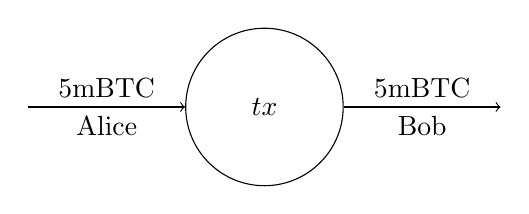
\begin{tikzpicture}
      \node[circle,draw, minimum size=2cm] (A) at (0,0) {$tx$};
      \draw [->] (-3,0) -- (A) node[midway, below]{Alice} node[midway, above]{5mBTC};
      \draw [->] (A) -- (3, 0) node[midway, below]{Bob} node[midway, above]{5mBTC};
    \end{tikzpicture}
    \caption{A bitcoin transaction}
    \label{fig:bl_tx:tx}
  \end{subfigure}
  \begin{subfigure}[t]{0.50\textwidth}
    \centering
    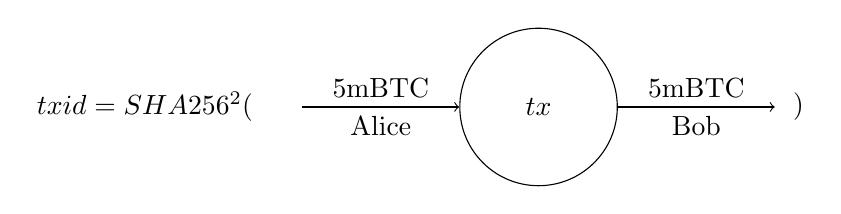
\begin{tikzpicture}
      \node[circle,draw, minimum size=2cm] (A) at (0,0) {$tx$};
      \draw [->] (-3,0) -- (A) node[midway, below]{Alice} node[midway, above]{5mBTC};
      \draw [->] (A) -- (3, 0) node[midway, below]{Bob} node[midway, above]{5mBTC};
      \node (txid) at (-5,0) {$txid = SHA256^{2}($};
      \node (txid) at (3.3,0) {$)$};
    \end{tikzpicture}
    \caption{Bitcoin Transaction ID}
    \label{fig:bl_tx:id}
  \end{subfigure}
  \caption{Transactions}
  \label{fig:bl_transaction}
\end{figure}

Payments are done throught linking transaction nodes and money is a chain of transactions. All transactions together form a transaction graph which is public and everyone participating in
the network can see and add new transactions to the graph. Spendable money are outgoing unlinked edges which are called unspent transaction outputs (UTXO). So for a user to spent her money
she has to claim her UTXO's, meaning to find all the UTXO that have her public key as recipient given she has the corresponding secret key. A user too spent money, first she find a transaction
that has a UTXO of which she is the owner. Then she creates one transaction with one incoming and one outgoing edge and connect the incoming edge of the new transaction with the old UTXO.
Now the old UTXO is not a UTXO anymore, it was just spent, and the outgoing edge of the new tx is unconnected and becomes the new UTXO. Finally she specifies the value and the owner (address)
of the new outgoing edge.


\begin{figure}[ht!]
    \centering
    \begin{tikzpicture}[scale=0.9]
      \node[circle,draw, minimum size=2cm] (A) at (0,0) {$tx$};
      \node[circle,draw, minimum size=2cm] (B) at (4,0) {$tx$};
      \node[circle,draw, minimum size=2cm] (C) at (8,0) {$tx$};
      \draw [->] (-3,0) -- (A) node[midway, below]{Alice} node[midway, above]{1mBTC};
      \draw [->] (A) -- (B) node[midway, below]{Bob} node[midway, above]{1mBTC};
      \draw [->] (B) -- (C) node[midway, below]{Charlie} node[midway, above]{1mBTC};
      \draw [->] (C) -- (11,0) node[midway, below]{Eve} node[midway, above]{1mBTC};

      \node[red] (D) at (10, 3) {$utxo$};
      \draw [->, red] (D) -- (10,0.8);
      \node[ellipse, draw, red, inner xsep=4.5ex,inner ysep=1.9ex] at (10,0) {};
    \end{tikzpicture}
  \caption{Transaction graph and UTXO}
  \label{fig:bl_utxo}
\end{figure}

\begin{figure}[ht!]
  \begin{subfigure}[t]{0.50\textwidth}
    \centering
    \begin{tikzpicture}
      \node[circle,draw, minimum size=2cm] (A) at (0,0) {$tx$};
      \draw [->] (A) -- (3,0) node[midway, below]{Alice} node[midway, above]{1mBTC};

      \node[red] (utxo) at (2, 3) {$utxo$};
      \draw [->, red] (utxo) -- (2,0.8);
      \node[ellipse, draw, red, inner xsep=4.5ex,inner ysep=1.9ex] at (2,0) {};
    \end{tikzpicture}
    \caption{Alice finds one UTXO that belongs to her}
    \label{fig:bl_spent:a}
  \end{subfigure}
  \begin{subfigure}[t]{0.50\textwidth}
    \centering
    \begin{tikzpicture}[scale=0.9]
      \node[circle,draw, minimum size=2cm] (A) at (0,0) {$tx$};
      \draw [->] (A) -- (3,0) node[midway, below]{Alice} node[midway, above]{1mBTC};
      \node[circle,draw, minimum size=2cm] (B) at (5,0) {$tx$};
      \draw [->] (B) -- (8,0) node[midway, below]{Bob} node[midway, above]{1mBTC};

      \node[red] (utxo) at (2, 3) {$utxo$};
      \draw [->, red] (utxo) -- (2,0.8);
      \node[ellipse, draw, red, inner xsep=4.5ex,inner ysep=1.9ex] at (2,0) {};
    \end{tikzpicture}
    \caption{Alice create a transaction with recipient Bob}
    \label{fig:bl_spent:b}
  \end{subfigure}
  \begin{subfigure}[t]{0.50\textwidth}
    \centering
    \begin{tikzpicture}[scale=0.9]
      \node[circle,draw, minimum size=2cm] (A) at (0,0) {$tx$};
      \node[circle,draw, minimum size=2cm] (B) at (4,0) {$tx$};
      \draw [->] (A) -- (B) node[midway, below]{Alice} node[midway, above]{1mBTC};
      \draw [->] (B) -- (7,0) node[midway, below]{Bob} node[midway, above]{1mBTC};

      \node[red] (utxo) at (2, 3) {$not\text{ }utxo\text{ }anymore$};
      \draw [->, red] (utxo) -- (2,0.8);
      \node[ellipse, draw, red, inner xsep=4.5ex,inner ysep=1.9ex] at (2,0) {};

      \node[blue] (utxo) at (6, 3) {$new\text{ }utxo$};
      \draw [->, blue] (utxo) -- (6,0.8);
      \node[ellipse, draw, blue, inner xsep=4.5ex,inner ysep=1.9ex] at (6,0) {};
    \end{tikzpicture}
    \caption{Alice connects the incoming edge of the new transaction with the old UTXO}
    \label{fig:bl_spent:c}
  \end{subfigure}
  \begin{subfigure}[t]{0.50\textwidth}
    \centering
    \begin{tikzpicture}[scale=0.9]
      \node[circle,draw, minimum size=2cm] (A) at (0,0) {$tx$};
      \node[circle,draw, minimum size=2cm] (B) at (4,0) {$tx$};
      \draw [->] (A) -- (B) node[midway, below]{Alice} node[midway, above]{1mBTC};
      \draw [->] (B) -- (7,0) node[midway, below]{Bob} node[midway, above]{1mBTC};

      \node[red] (utxo) at (4.8, 3) {$Alice\text{ }signs\text{ }$};
      \node[ellipse, draw, red, inner xsep=8ex,inner ysep=4ex] (ell) at (4.8,0) {};
      \draw [->, red] (utxo) -- (ell);
    \end{tikzpicture}
    \caption{Alice signs the transaction. No one else can forge this signature}
    \label{fig:bl_spent:d}
  \end{subfigure}
  \caption{Speding money}
  \label{fig:bl_spent}
\end{figure}

\subsection{Block}\label{blockchain:structure:block}

To prevent double-spending~\cite{wiki:double_spend,bitcoin_wiki:double_spend} the transaction must be put in chronological order so that it can be answered
if transaction A happen before transaction B. Furthermore, the order must be common for everyone in the network.
This global aggrement on a common truth is named consensus (§~\ref{blockchain:consensus_mechanisms}) and this is where the bitcoin novelty is.

A block contains many transactions and it cannot contain double spends;transactions that spend the same output.
Each transaction can appear only once in a block and a transaction in a valid block is called confirmed.

In bitcoin network a block is set to be created approximately one every ten minutes and every newly created block contains the most recent transactions that did not
exist in previous blocks. As in transaction every bitcoin block has a unique block id which comes from the double hash of the header of the block with the use of SHA-256 cryptographic hash function.

\begin{figure}[ht!]
  \begin{subfigure}[t]{0.50\textwidth}
    \centering
    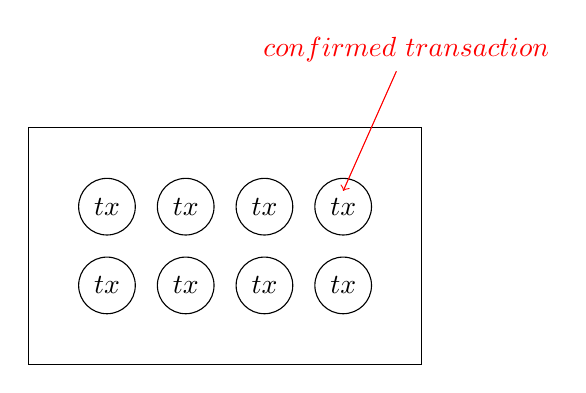
\begin{tikzpicture}
      \draw (0,0) rectangle (5,3);
      \foreach \x in {1,2,...,4}
        \foreach \y in {1,...,2}
          \node[circle,draw, minimum size=0.4cm] at (\x,\y) {$tx$};

      \node[red] (confirm) at (4.8, 4) {$confirmed \text{ }transaction$};
      \draw [->, red] (confirm) -- (4,2.2);
    \end{tikzpicture}
    \caption{A block}
    \label{fig:block:a}
  \end{subfigure}
  \begin{subfigure}[t]{0.50\textwidth}
    \centering
    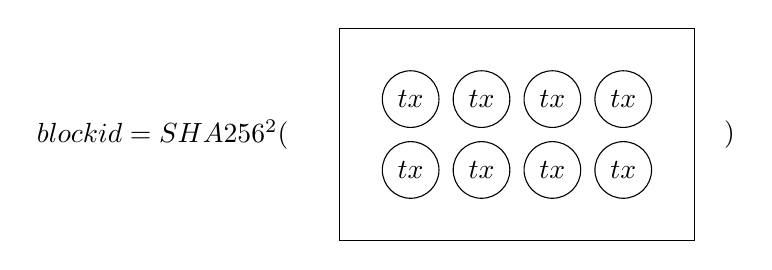
\begin{tikzpicture}[scale=0.9]
      \draw (0,0) rectangle (5,3);
      \foreach \x in {1,2,...,4}
        \foreach \y in {1,...,2}
          \node[circle,draw, minimum size=0.4cm] at (\x,\y) {$tx$};
      \node (txid) at (-2.5,1.5) {$blockid = SHA256^{2}($};
      \node (txid) at (5.5,1.5) {$)$};
    \end{tikzpicture}
    \caption{Bitcoin Block ID}
    \label{fig:block:b}
  \end{subfigure}
  \caption{Blocks}
  \label{fig:blocks}
\end{figure}

\subsection{Blockchain}\label{blockchain:structure:blockchain}

The blockchain data structure is an ordered back-linked list of blocks of transactions. Each block references a
previous block, known as the parent block, through a pointer to the previous block id. A later block cannot contain a double spend of a previous one or a transaction that appeared in a previous block.
So, a transaction A precedes transaction B if A is contained in a previous block from B and if we want to ensure that a transaction will not be double spent, we have to
wait for it to be confirmed. So, the need of a consensus-a single universal “truth”, a global aggrement- on the order of the blocks emerge (§~\ref{blockchain:consensus_mechanisms}).

\begin{figure}[ht!]
  \centering
  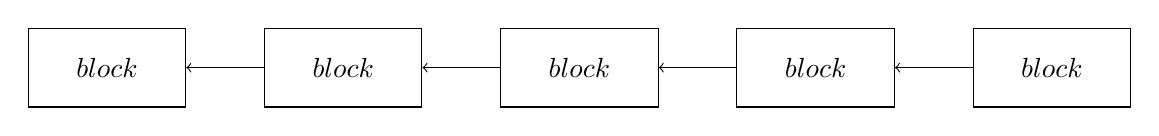
\begin{tikzpicture}
    \foreach \x in {0,1,...,4}
        \pgfmathparse{(\x*3)}
        \edef\position{\pgfmathresult}
        \node[rectangle,draw,minimum width=2cm,minimum height=1cm] (\x) at (\position,0) {$block$};

    \foreach \x in {1,2,...,4}
        \pgfmathparse{(\x-1)}
        \edef\previous{\pgfmathresult}
        \draw [->] (\x) -- (\previous);

  \end{tikzpicture}
  \caption{Blockchain}
  \label{fig:blockchain}
\end{figure}

\begin{figure}[ht!]
  \begin{tikzpicture}
    \foreach \x in {0,1,...,4}{
        \pgfmathparse{(\x*3)}
        \edef\position{\pgfmathresult}
        \node[rectangle,draw,minimum width=2cm,minimum height=1cm] (\x) at (\position,0) {$block$};
        \pgfmathparse{int(\x*10 + 10)}
        \edef\time{\pgfmathresult}
        \node[] at (\position,-2) {$17:\time$};
    }


    \foreach \x in {1,2,...,4}
        \pgfmathparse{(\x-1)}
        \edef\previous{\pgfmathresult}
        \draw [->] (\x) -- (\previous);

    \node[ellipse, draw, red, inner xsep=6ex,inner ysep=3ex] (old_ell) at (0) {};
    \node[ellipse, draw, red, inner xsep=6ex,inner ysep=3ex] (recent_ell) at (4) {};
    \node[red,below=0cm of old_ell] (old) {$oldest\text{ }block\text{ }$};
    \node[red,below=0cm of recent_ell] (recent) {$recent\text{ }block\text{ }$};
  \end{tikzpicture}
  \caption{Blockchain timeline}
  \label{fig:blockchain_timeline}
\end{figure}

\section{Consensus mechanisms}\label{blockchain:consensus_mechanisms}

The consensus mechanism is the core mechanism of the blockchain. Through consensus, the shared state of the ledger comes to an agreement upon a global state,
allowing all the nodes of the network to reach the same ledger state. Achieving consensus in a distributed system is challenging.
A consensus mechanism has to be resilient to node failures, network delays and the existence of malicious nodes~\cite{wiki:byzantine_fault_tolerance}.

There are three basic consensus mechanism categories:

\begin{enumerate}
  \item Proof-of-Work (PoW).
  \item Proof-of-Stake (PoS).
  \item Practical Byzantine Fault Tolerance (PBFT)
\end{enumerate}


\subsection{Proof of Work (PoW)}\label{blockchain:consensus:pow}

In the case of Proof-of-Work consensus mechanism, each network node participating in
the consensus tries to solve a computational puzzle that is computational hard, but feasible to find, and easy to verify correctness.
A PoW system is also based on randomness, which is approximated proportionally to the computational power of each node.
The participating nodes are bound to trial and error until a correct answer is found. Being a blockchain system a random node is selected as a winner for block creation.
In order for a block to be accepted by the rest of consensus participants, they must complete a proof of work based on the data of the block.
The difficulty of the work is adjusted in a way that a new block is generated in a specific time interval on average.

The process of solving a PoW computational puzzle is known as mining and the participants as miners.
The first miner that solves the puzzle gets to add the proposed block to the blockchain and broadcast
the block to the entire network. Due to network latency and the distributed nature of the system it is possible that two miners will
find a block around the same time and some nodes will accept the first block and some others the second one. In such cases there is a temporary
fork in the blockchain, where one node is adding blocks to one branch while other nodes are adding blocks to another branch. Eventually the
system will come to an agreement, the longest branch will be accepted and the others will be discarded.

Bitcoin~\cite{Zohar:2015:BUH:2817191.2701411} is the first blockchain system that utilizes a PoW for blockchain block generation. Due to the nature of PoW, bitcoin is vulnerable to 51\% attacks.
This means that if a node or a group of nodes is able to control over 51\% of the computational power of the network, it is able to manipulate
the verification process: by writing its own blocks, it has made it possible to double-spend funds or reject certain transactions.

PoW consensus mechanism works very well in public blockchain systems where trust of the nodes is low eliminating
the double-spend problem -to redirect previously processed payments and use the same money twice- and guarding against Sybil attacks~\cite{Vu:2009:PCP:1671222}.
However, the transaction confirmation time is longer compared to conventional financial services (such as VISA)\cite{Sompolinsky2015,Zohar:2015:BUH:2817191.2701411,DBLP:journals/corr/abs-1708-05665} resulting
in slower transaction confirmation rates. Lastly, the energy waste attributed to the mining process can be very high -the energy requirements
of the Bitcoin protocol are estimated to be comparable to those of a small country~\cite{6912770}.

\subsection{Proof of Stake (PoS)}\label{blockchain:consensus:pos}

Proof-of-Stake algorithms are designed to overcome the disadvantages of PoW in terms of the high electricity consumption involved in mining~\cite{bl_consensus}
and provide equal security guarantees~\cite{Kiayias2017}. Unlike PoW where the miners solve computational puzzles in order to create a new block, in PoS the choice
of the block creator among the miners is random, yet relative to the stake the miner possesses according to the current blockchain ledger. Maintaining
the blockchain relies on the stakeholders themselves and assigns work to them based on the amount of stake that each possesses as reported in the ledge~\cite{Kiayias2017}.
The higher the stake participant, the higher the possibility to be chosen.

Proof-of-Stake algorithms suffer from the so-called “nothing at stake” problem.
The “nothing at stake” problem refers to attacks against PoS blockchain systems where shareholders do not have
incentives to follow the protocol and vote simultaneously on multiple blockchains exploiting the fact that little computational effort
is needed to build a PoS blockchain~\cite{Kiayias2017}. Ouroboros is the first provable secure PoS algorithm~\cite{Kiayias2017} and is the main consensus algorithm of the Cardano blockchain~\cite{cardano_site}.

\subsection{Practical Byzantine Fault Tolerance (PBFT)}\label{blockchain:consensus:PBFT}

The Practical Byzantine Fault Tolerance algorithm~\cite{Castro:1999:PBF:296806.296824} is the first practical consensus algorithm with Byzantine Fault Tolerance~\cite{wiki:byzantine_fault_tolerance}.
It is based on the concept of state machine replication and replication state voting, and is able to process tens of thousands of requests per second with minimal latency.
The algorithm has only a 3\% overhead over a typical filesystem~\cite{Castro:1999:PBF:296806.296824}.

PBFT and state-machine replication protocols’ downside is related to scalability, in terms of the number of nodes (replicas)~\cite{Vukolić2016} that can be supported.
PBFT has only been scaled and studied up to 20 replicas~\cite{bl_consensus,Vukolić2016}. To overcome this limitation, without compromising security, various PBFT variants,
such as Ripple and Stellar, partition the network into smaller groups called federates and each one runs a local consensus protocol among its members and
global consensus is achieved when certain conditions are being met~\cite{DBLP:journals/corr/abs-1708-05665}.

\begin{table}[]
  \centering
  \resizebox{\textwidth}{!}{
    \begin{tabular}{|l|l|l|l|}
      \hline
      & PoW &	PoS &	PBFT \\ \hline
      Blockchain Type &	Permissionless &	Both &	Permissioned \\ \hline
      Scalability of nodes &	High &	High &	Low \\ \hline
      Scalability of clients &	High &	High &	High \\ \hline
      Transaction rate &	Low &	High &	High \\ \hline
      Latency &	High &	Low &	Minimal \\ \hline
      Power consumption &	High &	Low &	Low \\ \hline
      Token needed &	Yes &	Yes &	No \\ \hline
      Cost of participation &	Yes &	Yes &	No \\ \hline
      Adversary tolerance &	<= 25\%	& Depends &	<= 33\% \\ \hline
    \end{tabular}
  }
  \caption{Blockchain consensus mechanisms. Adapted and modified from~\cite{bl_consensus,Vukolić2016}}
  \label{table:blockchain_consensus}
\end{table}

\section{Incentives}\label{blockchain:incentives}

For miners to participate in the network and contribute their computation resources incentives must be provided.
Normally, in permissionless blockchains such as Bitcoin or Ethereum a monetary incentive in the form of cryptocurrency
incentivize the miners and in a permissioned blockchain finance incentives or access to blockchain data could encourage miners to participate~\cite{deloitte}.

\section{Blockchain Types}\label{blockchain:blockchain_types}

There are various types of blockchains varying in restrictions on data access and participation in the consensus process.
Each one has its own advantages and disadvantages.

\begin{itemize}
  \item Public Blockchain: A public blockchain is a blockchain, in which there are no restrictions on reading blockchain data -encrypted or not- and validating transactions~\cite{prbc_vs_pubbc}.
  The most common implementation of a public blockchain is Bitcoin~\cite{nakamoto2012bitcoin} and Ethereum~\cite{ethash}.
  \item Federated or Consortium blockchain: In a federated blockchain transaction validation is limited to a predefined list of entities with their identities known to the network. Data access can either be public or restricted~\cite{prbc_vs_pubbc}.
  \item Private blockchain: A private blockchain is a blockchain where consensus mechanism is centralized to one single entity regardless of data access~\cite{prbc_vs_pubbc}.
\end{itemize}

\section{Consensus defined types of Blockchain}\label{blockchain:consensus_blockchain_types}

\begin{itemize}
  \item Permissionless blockchain: A permissionless blockchain is a blockchain, in which there are no restrictions on identities of transaction processors (i.e., users that are eligible to create blocks of transactions)~\cite{prbc_vs_pubbc}.
  \item Permissioned blockchain: A permissioned blockchain is a blockchain, in which transaction processing is performed by a predefined list of subjects with known identities~\cite{prbc_vs_pubbc}.
\end{itemize}

\begin{table}[]
  \centering
  \resizebox{\textwidth}{!}{
    \begin{tabular}{|l|l|l|l|}
      \hline
       & Public & Permissioned (Multiple Entities) & Private (Single Entity) \\ \hline
       Participants & Permissionless - Anonymous & Permissioned - Identified, Trusted & Permissioned - Identified, Trusted \\ \hline
       Data Access & Public & Public or Restricted & Restricted \\ \hline
       Consensus & PoW, PoS & FBTA, PoS & FBTA \\ \hline
    \end{tabular}
  }
  \caption{Blockchain Types. Source~\cite{hub-bl-types}}
  \label{table:blockchain_types}
\end{table}

\section{Blockchain Implementations}\label{blockchain_implementations}

\subsection{Bitcoin}\label{blockchain:impl:bitcoin}
\subsection{Ethereum}\label{blockchain:impl:ethereum}

Ethereum is an open-source, public, blockchain-based distributed computing platform featuring smart contract functionality.
It provides a decentralized Turing-complete virtual machine, the Ethereum Virtual Machine (EVM), which can execute scripts using an
international network of public nodes~\cite{wiki:ethereum}. Ethereum provides a cryptocurrency called ether which can be transferred between accounts and gas,
an internal pricing mechanism used to execute contracts and allocate resources on the network. Through EVM, Ethereum provides Solidity a
Turing-complete language for writing smart contracts that enables anyone to build distributed applications making the process much easier and efficient than ever before.
Ethereum use a Proof-of-Work consensus mechanism called Ethash and has been designed to be ASIC-resistant~\cite{ethash}.
Soon Ethereum will be moved to a Proof-of-Stake consensus mechanism called Casper. Ethereum can be implemented as well as a permissioned blockchain~\cite{consortium_chain_development,quorum}.


\subsection{Hyperledger}\label{blockchain:impl:hyperledger}

Hyperledger is an open-source permissioned blockchain and provides a flexible, modular and secure architecture with a
pluggable consensus mechanism is among the most popular permissioned blockchains~\cite{DBLP:journals/corr/abs-1708-05665}. In Hyperledger, Fabric a predefined list of
entities is not only known, but their identities and roles are registered and verified with a central registry service running within the system.
It also supports smart contracts on the blockchain, also known as chaincode~\cite{bl_consensus} and does not support a cryptocurrency system. The default consensus
mechanism of Hyperledger is the Practical Byzantine Fault Tolerance algorithm (PBFT) which assumes authenticated nodes.
Hyperledger version 0.6 fails to scale up to more than 16 nodes~\cite{DBLP:journals/corr/abs-1708-05665} but version 1.0 architecture has been designed to address transaction and
node scalability in a manner adherent with regulatory and industry standard~\cite{imb_hypeledger_adv}.

\subsection{Cardano}\label{blockchain:impl:cardano}

Cardano is a security focused blockchain that utilize the latest research and engineering insights to build a platform suitable for
the highest value applications~\cite{cardano_site}. It supports distributed applications creation and smart contracts verifiable by a method called formal
verification allowing logical proof of correctness of code providing high security. Cardano addresses the need for regulatory oversight while
maintaining consumer privacy and security. Cardano is the first blockchain project to be peer reviewed by academic researchers~\cite{cardano_site} and its consensus
mechanism, Ouroboros, is the first Proof of Stake algorithm to be provably secure~\cite{Kiayias2017}.
Cardano consists of two main layers, one for accounting and one for computation. The accounting layer is called Cardano Settlement Layer (CSL)
and the computation layer Cardano Computation Layer (CCP) where distributed application can be built and run upon. The CCP layer has not been
implemented yet and there is a plan to be released as a beta by the first quarter of 2018~\cite{cardano_parsons}.

\subsection{Enigma}\label{blockchain:impl:enigma}

Enigma is a decentralized computation platform with guaranteed privacy~\cite{DBLP:journals/corr/ZyskindNP15}. It operates through a peer-to-peer network enabling
different parties to store and run computation on data while keeping privacy. Enigma uses a highly optimized version of secure multi-party computation (MPC)
guaranteed by a verifiable secret-sharing scheme~\cite{DBLP:journals/corr/ZyskindNP15}. A blockchain is utilized as the controller of the network, managing access to the data and identities.
The data are stored off-chain, encrypted in a distributed database, and a modified distributed hash table (DTH), accessible through the blockchain, is used for holding only references to the data.

%!TEX root = ../thesis.tex
\chapter{Smart Contracts}
\label{smart_contracts}

A smart contract is a computer protocol intended to facilitate, verify, or enforce the negotiation or performance of a contract~\cite{FM548,wiki:smart_contract}.
The idea of smart contracts proposed in the early 1990s~\cite{FM548} and have been used primarily in association with cryptocurrencies enabling
parties to formally specify a cryptographically enforceable agreements~\cite{7163021}.

Bitcoin offers smart contracts through a stack-based scripting language that is not Turing-complete limiting the type of smart contracts one can create.
Numerous previous smart contract application atop Bitcoin (e.g., lottery\cite{Andrychowicz:2014:SMC:2650286.2650764,10.1007/978-3-662-44381-1_24},
verifiable computation~\cite{Kumaresan:2014:UBI:2660267.2660380}) have demostrated the difficulty of Bitcoin's scripting language~\cite{cryptoeprint:2015:675}.

Ethereum is the first Turing-complete decentralised smart contract framework. With Ethereum launch, the notion of DApps (decentralized applications) arised
and a lot of developers and companies are building numerous applications atop Ethereum such as prediction markets~\cite{augur,gnosis}, social media platforms~\cite{akasha,backfeed},
online gambling~\cite{etheroll,coinpoker} and video games~\cite{cryptokitties}. As of January 2018, there are more than 250 live DApps,
with hundreds more under development~\cite{wiki:ethereum}.

\section{Consent}
\label{smart_contract:consent}

Modeling dynamic consent in smart contracts should be carefully analyzed taking into account design issues that are related to smart contracts lifecycle, required state variables for storing contract’s information, and access restrictions to those variables.

Neisse et al.~\cite{DBLP:journals/corr/NeisseSF17} proposed the following three models for data accountability and provenance tracking that comply with the GDPR~\cite{gdpr}:

\begin{enumerate}
  \item Contract for a specific controller: A contract where the data subject creates a contract tailored for each data controller
  \item Contract for specific data: A contract where each subject’s data instance is shared among all data controllers
  \item Contract for multiple data subjects: A contract where the data controller specifies how the data from all subjects are treated from the controller
\end{enumerate}

The first contract is more adequate for sensitive data~\cite{DBLP:journals/corr/NeisseSF17}, such as health data, since a subject-controller relationship~\cite{Azaria2016} is being created where each patient has a different contract for each controller accessing their data, providing fine grained access control and provenance information. On the other hand, it has the highest cardinality among the others two types~\cite{DBLP:journals/corr/NeisseSF17}. The second contract suffers from direct linkability as a unique subject address is needed compromising patients’ privacy~\cite{DBLP:journals/corr/NeisseSF17}. Lastly, the third one has the lowest cardinality among the others but also has the lower level of customization due to the limited number of contract options~\cite{DBLP:journals/corr/NeisseSF17}.

%!TEX root = ../thesis.tex
\chapter{Off chain computation}
\label{off_chain}

\section{Secure multi-party computation}\label{off_chain:mpc}

%!TEX root = ../thesis.tex
\chapter{Zero Knowledge Proofs}
\label{zkp}

A proof of knowledge is a protocol that enables one party to convince another of the validity of a statement.
In a zero-knowledge proof, this is accomplished without revealing any information beyond the legitimacy of the proof~\cite{kiagias:crypto},
meaning that one party can prove to another party that a given statemnet is true, without conveying any information apart from
the fact that the statement is indeed true~\cite{wiki:zkp}.

Let $\calp$ be a prover and $\calv$ the verifier. $\calp$ must convince $\calv$ that she has some
knowledge of a statement $x$ without explicitly stating what she knows. We call this knowledge a witness $w$.
Both parties are aware of a predicate $R$ that will attest to $w$ being a valid witness to $x$~\cite{kiagias:crypto}. In general,

\begin{itemize}
  \item The predicate $R$ is assumed to be polynomial-time computable.
  \item The prover $\calp$ has $R,x$, and $w$ such that $R(x,w) = 1$. She wishes to prove possesion of $w$ by producing a proof of knowledge $\pi$.
  \item The verifier $\calv$ has $R,x$, and $\pi$.
  \item Given $R$ it is hard to find a corresponding $w$ such as $R(x,w) = 1$
  \item The prover $\calp$ is reluctant to reveal $w$; otherwise the solution is trivial.
  \item The verifier $\calv$ can efficiently check the validity of $\pi$.
\end{itemize}

\section{Examples}

\subsection{The strange cave of Ali Baba}
\label{zkp:examples}

Suppose there is our old friends Alice and Bob. At the bottom of the cave~\cite{Quisquater:1989:EZP:118209.118269} of figure~\ref{fig:zkp:alibaba} there is a magic door that
can only be open using a secret password. The cave is shaped like a rentacle with one entrace at one side and the magic door blocking the opposite side.
Bob knows the secret password and wants to prove to Alice that he can open the magic door without revealing the password to Alice.
Bob propose the following game to prove to Alice he can open the magic door: Alice waits outside the cave, Bob enters the cave and
takes either left or right path. Alice can not see which path Bob takes. Then Alice enters, stants at the entrance of cave and calls
Bob to come out either the left or the right passage. Bob complies, using the secret password if necessary.

If Bob does not know the secret password he has $1/2$ change of guessing correctly (he would only be able to return by the named path if
Alice were to give the name of the same path by which he had entered) as Alice choose at random which path Bob should take. If they repeat this procedure
$k$ times the probability of Bob convincing Alice that he knows the secret password without actually knowing it reduce exponetially. In particular, at most $1/2^{k}$.

\subsection{The colour-blind friend}

Let's bring again our friends Alice and Bob. Suppose Bob is color-blind~\cite{wiki:zkp,zkp:colour_blind} and Alice has two balls: one red and one green but otherwise identical when you touch them.
To Alice they seem complete identical and she is not sure if they are actually distinguishable. Bob wants to prove to Alice that indeed the are differently-coloured
without revealing which one is red and which is green. To prove his knowledge, Bob gives to Alice the two balls so that she is holding one in each hand. Bob can see
at this point which ball is in which hand. Next, Alice either switches the ball behind her hands or leaves them be, with probability $1/2$. Finally, she brings
them out from behind her back. Alice then asks Bob if she switch the balls. By looking at their colors, Bob can can say with certainty whether he switched them or not.
On the other hand, if they were the same color and hence indistinguishable, there is no way you could guess correctly with probability higher than 1/2. If they repeat
this procedure $k$ times the probability that Bob succeeded at identifying all the switch/non-switches when the balls are identical (thus lying to Alice) is at most
$1/2^{k}$.

\begin{figure}[t!]
  \centering
  \begin{subfigure}[t]{0.30\textwidth}
    \centering
    \resizebox{\linewidth}{!}{
      \begin{tikzpicture}[scale=1]
        % Cave %
        \draw(0,5) -- (2,5) -- (2,8) -- (10,8) -- (10,4);
        \draw(0,4) --(2,4) -- (2,1) -- (10,1) -- (10, 4);
        \draw(9,4.5) -- (10,4.5);
        \draw(3,5) -- (3,7) -- (9,7) -- (9,5);
        \draw(3,5) -- (3,2) -- (9,2) -- (9,5);
        % Actors %
        \draw[fill] (1,5.6) circle [radius=0.1];
        \node [below] (alice) at (1,5.5) {Alice};
        \draw[fill] (2.5,4.6) circle [radius=0.1];
        \node [below] (bob) at (2.5,4.5) {Bob};
        % Arrows %
        \draw [dashed, ->] (2.5,4.6) -- (2.5,6);
        \draw [dashed, ->] (2.5,3.9) -- (2.5,2);

      \end{tikzpicture}
    }
    \caption{Alice stands outside and Bob choose randomly a path, left or right}
    \label{fig:zkp:alibaba:a}
  \end{subfigure}
  \begin{subfigure}[t]{0.30\textwidth}
    \centering
    \resizebox{\linewidth}{!}{
      \begin{tikzpicture}[scale=1]
        % Cave %
        \draw(0,5) -- (2,5) -- (2,8) -- (10,8) -- (10,4);
        \draw(0,4) --(2,4) -- (2,1) -- (10,1) -- (10, 4);
        \draw(9,4.5) -- (10,4.5);
        \draw(3,5) -- (3,7) -- (9,7) -- (9,5);
        \draw(3,5) -- (3,2) -- (9,2) -- (9,5);
        % Actors %
        \draw[fill] (2.5,4.6) circle [radius=0.1];
        \node [below] (alice) at (2.5,4.5) {Alice};
        \draw[fill] (9.5,4.3) circle [radius=0.1];
        \node [below] (bob) at (9.5,4.2) {Bob};
        % Speech Bubble %
        \node[overlay,draw,cloud callout,callout relative pointer={(0.2cm,-0.7cm)},%
        aspect=2.5,fill=white!90] at ($(alice)+(-0.5cm,2.3cm)$) {Left};

      \end{tikzpicture}
    }
    \caption{Alice calls to Bob, asking him to come out either the left or the right passage}
    \label{fig:zkp:alibaba:b}
  \end{subfigure}
  \begin{subfigure}[t]{0.30\textwidth}
    \centering
    \resizebox{\linewidth}{!}{
      \begin{tikzpicture}[scale=1]
        % Cave %
        \draw(0,5) -- (2,5) -- (2,8) -- (10,8) -- (10,4);
        \draw(0,4) --(2,4) -- (2,1) -- (10,1) -- (10, 4);
        \draw(9,4.5) -- (9.5,4.5);
        \draw(3,5) -- (3,7) -- (9,7) -- (9,5);
        \draw(3,5) -- (3,2) -- (9,2) -- (9,5);
        % Actors %
        \draw[fill] (2.5,4.6) circle [radius=0.1];
        \node [below] (alice) at (2.5,4.5) {Alice};
        \draw[fill] (2.5,7.8) circle [radius=0.1];
        \node [below] (bob) at (2.5,7.7) {Bob};
        % Speech Bubble %
        \node[overlay,draw,cloud callout,callout relative pointer={(0.2cm,-0.7cm)},%
        aspect=2.5,fill=white!90] at ($(alice)+(-0.5cm,2.3cm)$) {OK};

      \end{tikzpicture}
    }
    \caption{Bob complies appearing at the exit Alices names}
    \label{fig:zkp:alibaba:c}
  \end{subfigure}
  \caption{Ali Baba Cave}
  \label{fig:zkp:alibaba}
\end{figure}

\section{Formal Definition}
\label{zkp:definition}

Let $<\calp, \calv>$ be a pair of interactive programs. Define $\text{out}^{\calp}_{\calp, \calv}(x,w,z)$
to be the output of $\calp$ when both $\calp$ and $\calv$ are executed with the public input $x$ and private
inputs $w$ and $z$ ($\calp$ determines $w$ and $\calv$ choose $z$); $\text{out}^{\calv}_{\calp, \calv}(x,w,z)$
is similar defined for $\calv$. The PPT interactive protocol $<\calp, \calv>$ is a \textbf{zero-knowledge proof}
for a language $L \in NP$ with knowledge error $k$ and zero-knowledge distance $\e$ if the following
properties hold~\cite{kiagias:crypto}.

\begin{enumerate}
  \item \textbf{Completeness:} If $x \in L$ and $R(x,w) = 1$ for some witness $w$, then $\text{out}^{\calv}_{\calp, \calv}(x,w,z)$ = 1
    for all string $z$ with overwhelming probability in $v$.
  \item \textbf{Soundness:} For any polynomial-time program $\calp^{*}$ define for arbitrary $x,w,z,$
    \begin{equation*}
      \pi_{x,w,z} = \Prob[\text{out}^{\calv}_{\calp^{*}, \calv}(x,w,z) = 1].
    \end{equation*}
    A protocol $<\calp, \calv>$ satisfies soundness if there are non-negligible functions $s(v), q(v)$ such for all $\calp^{*}$ here exists a probabilistic
    Turing machine (PTM) program $K$, called a knowledge extractor with the following property. Suppose that

    \begin{equation*}
      \widetilde{\pi} = \Prob[K(x,w,z) = w^{'} : R(x, x^{'}) = 1].
    \end{equation*}
    Then it holds that $\pi_{x,w,z} \geq s(|x|)$ implies that $\widetilde{\pi}_{x,w,z} \geq q(\abs{x})$.

  \item \textbf{(Statistical) Zero-knowledge:} For each polynomial-time program $\calv^{*}$, there is a PTM program $S$, called the \textbf{simulator}, such that for all
    $x,w$ with $R(x,w) = 1$, the random variables $S(x,z)$ and $\text{out}^{\calv^{*}}_{\calp, \calv^{*}}(x,w,z)$ are statistically indistinguishable for all strings $z$:
    \begin{equation*}
      \forall \cala \abs[\Big]{\Prob[\cala(S(x,z) = 1)] - \Prob[\cala(\text{out}^{\calv^{*}}_{\calp, \calv^{*}}(x,w,z)) = 1]} < \e.
    \end{equation*}
\end{enumerate}

Completeness is very similar to correctness. Assuming both the prover and verifier follow the protocol faithfully, completeness guarantees that the
protocol will succeed with a sufficiently high probability.
Soundness ensures that if the statement is false, no cheating prover can convince the honest verifier that it is true, except with some small probability.
Intuitively, statistical zero-knowledge is a property that prohibits a verifier from extracting information from an honest prover.
A weaker version of zero-knowledge is honest-verifier zero-knowledge (HVZK). Here it is assumed that the verifier executes the protocol faithfully,
but makes additional computations~\cite{kiagias:crypto}.

\section{zk-SNARKs}
\label{zkp:snarks}

Since computational power is often limited to devices such as mobiles or IoT (clients) the need of outsourcing computation to one or more powerful workers on the cloud emerges. Yet, confidence is needed at the working entity for proper computation. For this reason, the client should be able to verify the correctness of the results returned. That way not only the client is protected from malicious or malfunctioning workers but also the legitimate worker is benefit by shedding liability~\cite{pinocchio-nearly-practical-verifiable-computation}. This scheme is called public verifiable computation (VC).

In a public verifiable computation scheme the client outsource the evaluation of a function $F$ on input $u$ known to the client (e.g. a query). The client then can verify the correctness of the computation of $F(u)$ with less work than required for the computation of $F(u)$. When the outsource function $F$ consist of two inputs $u$ and $w$, where $w$ is the worker's private input (e.g a data set), then the scheme is a Zero-Knowledge Verifiable Computation (or non-interactive zero knowledge (NIZK) proof~\cite{Blum:1991:NZ:123137.123145}) if the client learns nothing about worker's input expect the output of the computation~\cite{pinocchio-nearly-practical-verifiable-computation}.

Such schemes are not interactive meaning no interaction is necessary between prover and verifier (worker and client) and a common reference string (CRS) shared between them is enough to achieve computational zero-knowledge~\cite{Blum:1991:NZ:123137.123145}.

Formally, as defined by Parno et. al~\cite{pinocchio-nearly-practical-verifiable-computation} a public Zero-Knowledge verifiable computation scheme $\calv \calc$ consist of a set of three polynomial-time algorithms:

\begin{itemize}
  \item $(EK_F, VK_F) \leftarrow \text{KeyGen}(F, 1^{\lambda})$: The randomized key generation algorithm. It takes as input the outsourced function $F$ and a security parameter ${\lambda}$; it outputs a public evaluation key $EK_F$ and a public verification key $VK_F$.
  \item $(y, \pi_y) \leftarrow \text{Compute}(EK_F, u)$: The deterministic worker algorithm. It takes as input the public evaluation key $EK_F$ and a public input $u$; it outputs $y \leftarrow F(u, w)$, where $w$ is an auxiliary private input, and a proof $\pi$ of $y$'s correctness.
  \item $\{0, 1\} \leftarrow \text{Verify}(VK_F, u, y, \pi_y)$:  The deterministic verification algorithm. It takes as input the public verification key $VK_F$, the public input $u$, the output $y$ and the proof $\pi_y$; It outputs $1$ if $F(u) = y$ and $0$ otherwise.
\end{itemize}

The acronym zk-SNARK stands for `Zero-Knowledge Succinct Non-Interactive Argument of Knowledge` in which each individual part, informally, have the following meaning~\cite{zksnarks_nutshell, zcash, 184425, Bitansky:2012:ECR:2090236.2090263}:

\begin{itemize}
  \item Zero-Knowledge: The verifier learns nothing but the validity of the computation
  \item Succinct: The proof are sort and easy to verify in comparison to the actual computation (constant size and polynomial verifiable in the size of the proof)
  \item Non-Interactive: There is no or little interaction done in one step. Anyone can verify without the need of interacting anew (publicly verifiable)
  \item ARgument: Soundness (§~\ref{zkp:definition}) holds only against computationally bounded provers
  \item of Knowledge: If the verifier accepts a proof output by a computationally bounded prover, then the prover has a witness for the given instance
\end{itemize}

At high level, zkSNARKs consist of four basic steps (Figure ~\ref{fig:zkp:zksnark_flow}):

\begin{enumerate}
  \item Computation to Arithmetic circuit~\cite{wiki:circuits}
  \item Arithmetic circuit to Rank 1 Constraint System (R1CS)~\cite{ggpr}
  \item R1CS to Quadratic Span Program (QAP)~\cite{ggpr}
  \item QAP to zkSNARK~\cite{pinocchio-nearly-practical-verifiable-computation}
\end{enumerate}

The main idea for constructing zkSNARKs is firstly to transform the generic program as a quadratic equation of polynomials (QAP)~\cite{ggpr}: $p(x)q(x) = s(x)r(x)$, where the equality holds if and only if the program is computed correctly. So the prover wants to convince the verifier that the equality holds.

Succinctness is achieved by random sampling. The verifier chooses a secret evaluation point $x_0$ to reduce the problem from polynomial multiplication and equality to simple number arithmetic checks: $p(x_0)q(x_0) = s(x_0)r(x_0)$. To allow the prover to compute the evaluation of the polynomials at $x_0$, without revealing $x_0$, Homomorphic encryption is used:  $E(p(x_0))E(q(x_0)) = E(s(x_0))E(r(x_0))$

Finally the prover obfuscates the encrypted values by multiplying with a number so that the verifier can still check the correctness of the structure without knowing the actual
encrypted values: $E(k + p(x_0))E(k + q(x_0)) = E(k + s(x_0))E(k + r(x_0))$

\begin{figure}[ht!]
  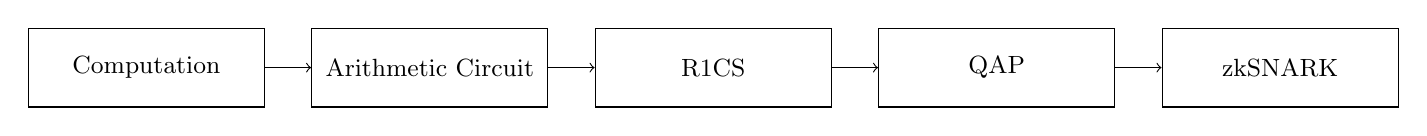
\begin{tikzpicture}[
    flow/.style={rectangle, minimum width=3cm, minimum height=1cm, text centered, draw=black,font=\small},
    scale=0.9
  ]
    \node[flow] (comp) at (0, 0) {Computation};
    \node[flow] (alg) at (4, 0) {Arithmetic Circuit};
    \node[flow] (r1cs) at (8, 0) {R1CS};
    \node[flow] (qap) at (12, 0) {QAP};
    \node[flow] (zk) at (16, 0) {zkSNARK};

    \draw[->] (comp) -- (alg);
    \draw[->] (alg) -- (r1cs);
    \draw[->] (r1cs) -- (qap);
    \draw[->] (qap) -- (zk);


  \end{tikzpicture}
  \caption{Steps of zk-SNARK}
  \label{fig:zkp:zksnark_flow}
\end{figure}

\note{Implementations of zksnark (pinnochio, Hawk, Zcash etc)}

%!TEX root = ../thesis.tex
\SetBlockThreshold{1}
\chapter{Problem Statement}
\label{problem}

The amount of data is rapidly increasing and it is estimated that 20\% of the world's data have been collected the past
few years~\cite{10.1109/SPW.2015.27,big_data_better_worse}. Data storage rapid growth contributes to a substantial shift in economy power and source of economic value. We have entered to the area of Big Data. The impact of Big Data is huge and the consequences are far reaching.

Data is a strategic asset that allows companies to be competitive. The value of raw data varies from a hundred cents to over several hundred dollars per individual~\cite{pr_data_cost_1, pr_data_cost_2, pr_data_cost_3}. The more is analyzed, modified and enriched, the more its value increasing.

People constantly producing and publishing data about themselves
leaving a constant moving digital fingerprint over the Internet; their personal data. The type, quantity and value of personal data
being collected are vast~\cite{emergence_new_assets_wef}: banks accounts, medical records, employment data, web searches, sites visited,
likes, dislikes, product purchase histories, quotes, tweets, texts, emails, phone calls, photos, videos, personal moments, emotions
as well as coordinations of real-world locations.

Personal data are gathered by few big tech companies being the rightful owners---personal data is owned by the institution that collects them---and privatizing them. This gave rise to the data broker and mining industry creating data marketplaces~\cite{dawex, q_dx, datastreamx} and trade platforms where data can be sold and bought for a price. All data is potentially for sale.

Personal data can be gathered as follows~\cite{emergence_new_assets_wef}:

\begin{itemize}
  \item Volunteered data: data shared explicitly by the individuals
  \item Observed data: data captured by recording actions of individuals
  \item Inferred data: data based on analysis of individuals volunteered or observed data
\end{itemize}

Big data can not exist without personal input and wide-scale cooperation. Free services by companies---in return for user input--- is an example of consumer-driven big data; leisure time transforms into productive work.

As some put it~\cite{data_new_oil_01,data_new_oil_02,data_new_oil_03,data_new_oil_04,data_new_oil_05,data_new_oil_05,data_new_oil_06,data_new_oil_07,data_new_oil_08,data_new_oil_09}: Data is the new oil.

Treating personal data as a natural resource is a huge problem and should be prevented.

The current centralized model in which third-parties collect and control massive amount of personal data should be questioned.
Individuals have little or no control over their personal data and how they are used growing that way a public concern about
user privacy.

Personal data should be in total control by the person that produce them, the rightful owner. Individuals should be empowered
with the ability to own their personal data, to control how are been collected, used, shared and by whom.

Nevertheless, the ability to process large volumes of personal information has still resulted in some benefits for individuals and society at large. Big data has positive implications for urban planners who want to design smarter cities, health-care professionals who want to predict epidemics and cure diseases, and engineers who want to identify or even predict new problems to solve.

\section{Regulations}\label{problem:regulations}

The EU directive 95/46/EC~\cite{eu-46ec-1995} defines personal data as follows:
\blockquote{
personal data shall mean any information relating to an identified or identifiable natural person ('data subject'); an identifiable person is one who can be identified, directly or indirectly, in particular by reference to an identification number or to one or more factors specific to his physical, physiological, mental, economic, cultural or social identity;
}
However there has been a clear notion that the data subject can potentially identified by pseudo-identifiers~\cite{wiki:pii}.
In the new General Data Protection Regulation (GDPR)~\cite{gdpr} by EU this has been formalised as:
\blockquote{
a data subject is one who can be identified, directly or indirectly, by means reasonably likely to be used by the controller or by any other natural or legal person
}

The recent approval of GDPR~\cite{gdpr} in 2016 by the European Commission (EC)
imposes new obligations on data controllers and processors in contrast to the previously adopted Data Protection Directive (DPR)~\cite{eu-46ec-1995}.
New legislation aims in the extension of responsibility and accountability requirements of organizations also demanding explicit
consent of the data subjects (person) securing their right to withdraw, and to be forgotten~\cite{DBLP:journals/corr/NeisseSF17}.

The key changes of the new data protection law introduced by the GDPR in contrast to the DPR is are~\cite{DBLP:journals/corr/NeisseSF17}:
\begin{itemize}
    \item Organisations based outside EU that process personal data of EU residents are applicable to the new legislation
    \item All EU member states are obliged to a single set of rules
    \item The responsibility and accountability requirements of organisations are extending
    \item EU residents are empowered with explicit consent over their data with the right to be forgotten
\end{itemize}

\section{OpenData}\label{problem:opendata}

\section{Motivations for applications}\label{problem:motivations}

banking, healthcare, national security, citizenship documentation or online retailing

%!TEX root = ../thesis.tex
\chapter{Solution}
\label{solution}

In our solution a public blockchain is used as the controller of the application. It is responsible for keeping an audit, immutable, tamper-proof and transparent log of all actions of the participants.

Blockchain does not provides an extra security layer concerning datasets. The datasets are stored off-chain, data controllers are responsible for the security of their system and the participants can still collaborate outside the Blockchain network. Nevertheless, the use of the Blockchain can guarantee accountability, auditability and provenance tracking of the data increasing the trust for the system.

\section{Participants}
\label{solution:entities}

There are three main roles consisting the application: the data controller, the data processor
and the data requester. The first two are also defined in the context of GDPR (§~\ref{problem:regulations}).
GDPR defines another role, that of data subject; the owner of the data.
In our scheme we assume that the data controller already has consent to access or forward the data or she is at the same time the data subject and the data controller.

\subsection{Data Controller}
\label{solution:entities:data_controller}

The data controller is in charge of a data set. It run on behalf of a data subject (person)
that authorizes the data controller to access its personal data, with the possibility of forwarding
them to a data processor that will be responsible for processing the data on behalf of controller~\cite{DBLP:journals/corr/NeisseSF17}.

\subsection{Data Processor}
\label{solution:entities:data_processor}

The data processor is responsible for processing data on behalf of the data controller. It listens for data processing requests and returns, along with the output of the process, a Zero Knowledge Proof of correct computation over the requested data set.

\subsection{Data Requester}
\label{solution:entities:data_req}

The requester can be any entity that requests a computation over a data set. It can be a research center, a university, a machine learning algorithm or any individual. The requester expects, along with the output, a proof of correct computation over the requested data set that verifies at the end of the processing.

\section{Threat model}
\label{solution:treat_model}

Before we explain in detail our architecture and the trust issues, we would like to introduce our thread model and what exactly our goals are. It is important to understand the possible roles of adversaries, their strengths and their resources.

In our model we assume a public blockchain where the involved entities that interact with a data set---the data controller and the data processor---are identified and verified through a public key infrastructure (PKI)~\cite{adams_understanding_2003}. Furthermore, each of the authenticated entities has certain trust properties. Τhe data controller is trusted for integrity and confidentiality and the data processor only for confidentiality.

Adversaries can be divided in 4 categories:

\begin{itemize}
  \item Malicious data controller
  \item Malicious data processor
  \item Malicious requestor
  \item Malicious public user
\end{itemize}

Each of these entities have different resources and goals. These are explained below.

\subsection{Malicious data controller}
\label{solution:treat_model:mcontroller}

A malicious data controller is a controller who tries to manipulate the results of the processing by either crafting fabricated datasets or working in collusion with the data processor. For example, an adversary could manipulate the dataset to make a classifier produce false negatives~\cite{dalvi2004adversarial} or the image representations in a deep neural network (DNN) to mimic those of other natural image~\cite{sabour2015adversarial}.

In our solution we do not address those issues. We assume that a data controller is honest and is authorized by a PKI that ensures the quality of the datasets.

\subsection{Malicious data processor}
\label{solution:treat_model:mprocessor}

As data controllers certain data processors may want to manipulate the results of the processing. A malicious data processor could influence the results of the processing with the following means:

\begin{itemize}
  \item Fake computation
  \item Process different dataset
  \item Use different algorithm
  \item Expose a dataset
\end{itemize}

We aim to fully protect requestors from such malicious actors except data disclosure.

\subsection{Malicious requestor}
\label{solution:treat_model:mrequestor}

The role of a requestor is certain: it can only make requests. Therefore, the only attack a malicious requestor can perform is a distributed denial-of-service attacks (DDoS) by flooding the network with requests in an attempt to overload the data processors and prevent other requests from being fulfilled. DDoS attacks are not address in this work and are left for future work (§~\ref{future_work:incentives}). An easy solution is to introduce a scalable payment system where the requestor pays per byte processed.

\subsection{Malicious public user}
\label{solution:treat_model:mpublic_user}

As the blockchain is public, malicious external users should be taken into account. External actors can perform Sybil attacks~\cite{sybil_attack} by impersonating the various actors of the system. All the possible attacks that can be performed by the previous malicious actor they can also be performed by an external user. The PKI assumption prevents forging controller and processor identifies.

\section{Blockchain}
\label{solution:blockchain}

The use of a public blockchain keep track the actions of each participant of the system. Each action is logged in the blockchain, a log that is immutable and irreversible. Blockchain serves as a public bulletin board where there is an order in time the actions occur, no one can alter or modify the records and every action can be auditable by anyone. This way, each entity is accountable for each action which they cannot later deny. Blockchain also can provide dataset timestamping in a decentralized manner. The hash of the dataset can be stored in the blockchain, which serve as a secure proof of the creation and modification time of the dataset.

\section{Algorithms}
\label{solution:algorithms}

The system should support only a set of open-source algorithms that have been analyzed and constructed to be privacy-preserving with the use of techniques such as k-anonymity~\cite{Samarati98protectingprivacy} and l-diversity~\cite{Aggarwal2008}. This algorithms should return only de-identified aggregated results.

The supported algorithms are:

\begin{enumerate}
  \item Sum
  \item Average
  \item Count
  \item Maximum
  \item Median
  \item Minimum
\end{enumerate}

The above algorithms are not considered to be privacy-preserving as it is outside the scope of the initial prototype and should be implemented on future work(§~\ref{future_work:ppq}).

\section{Zero-Knowledge Verifiable Computation}
\label{solution:proof}

Every data processor provides a proof of correctness for the execution of a computation on a given dataset without revealing the dataset itself. As the processor is obligated to provide a proof---a rational verifier rejects a computation without it---it is impossible for the processor a) to pretend that it done a processing without actually make any computation at all; b) to process a different dataset of its choice; c) to execute a different algorithm other than the requested one. It is evident that a Zero-Knowledge proof of computation plays a crucial role as it address various threats by malicious processors and enforce them to be honest.

Constructions of zkSNARKs require a one-time trusted setup in which a common-reference string (CRS) is generated; the public parameters of the system. The CRS is used to construct and verify proofs. Proof generation and verification requires two publicly available keys which derived from the CRS: the evaluation key $ek_f$ and the verification key $vk_f$. For each of the available algorithms processors use, a trusted setup must be done to produce the key pair $(ek_f, vk_f)$. Anybody that can obtained the trapdoor information corresponding to the CRS can produce fake proofs. For that reason, whomever runs the setup should be trusted. Various alternatives to bypass the trusted party---such as secure multi-party computation for CRS generation~\cite{zcash_mpc} or multi-string models~\cite{groth2014cryptography} where a set of untrusted authorities generate a random trusted string---have been proposed. In our solution, we assume that the trusted entity, that registers and verifies the parties through the PKI, is also responsible for key generation and distribution. The distribution can be done either by saving the public parameters on the blockchain or in a publicly available server.

The processor executes an algorithm $F$ with public input $u$ and private input $w$. Using  the evaluation key $ek_f$ it generates a zero knowledge proof with which the requestor using the verification key $vk_f$ can verify that the processor executed the algorithm $F$ correctly with inputs $u$ and $w$.

First, the data processor want to prove to the verifier that the computation is indeed done on the requested dataset without disclosing the dataset to it. The dataset is the private input $w$. For better understanding of the construction of the proof we define a game where tree participants are involved: a trusted oracle, a  computationally bounded processor and a requestor. The trusted oracle has a list of datasets and their hashes. The oracle cannot cheat or collaborate with any of the participant and for the same dataset it produces the same hash. At any moment the oracle selects randomly a dataset, gives it to the processor and announce the hash of the dataset to the requestor. The requestor ask the processor to compute the hash of the dataset as a proof. The requestor accepts the proof if and only if the hash of the processor match the hash of the oracle and rejects otherwise. The processor is forced to correctly compute the hash of the dataset as it is the only way to convince the requestor; hash functions are one-way and the oracle is trusted. Let's modify our game and assume now that the oracle gives the hash of the dataset to both the processor and requestor. The processor can easily convince the requestor without computing the hash; it knows the hash beforehand. To countermeasure that, the requestor demands from the processor to produce a proof of verifiable computation. It gives as function $F$ the same hash function $H$ the oracle used and ask the processor to generate a proof for $F = H(h, d)$ where $d$ is the dataset given by the oracle and $h$ the hash of it. The hash is the public input $u$. As processor wants to disclose the dataset $d$ it produces a zero knowledge proof. The requestor verifies the proof and accept if and only if the proof is valid. Again, the processor can not done anything but to comply and computes the digest. The data controller combined with the blockchain acts as the trusted oracle. The data controller is trusted to publish in the correct digest of the dataset in the blockchain and the immutability property of it prevent a malicious processor to change the digest to its preferences.

What remains, is to include inside $F$ the processing procedure of the dataset. The algorithm $F$ with private inputs $d$ and public input $h$, for which a zero knowledge proof of correct computation is generated, consists of a) hash generation of dataset $d$; b) dataset processing.

Informally, let $d$ be a private dataset, $H$ a cryptographic hash function and $h = H(d)$ the digest of $d$ over $H$. Let $\calp$ be a prover (data processor) and $\calv$ the verifier (data requestor). Prover $\calp$ produces a zkSNARK proof (§~\ref{zkp:snarks}) $\pi$ for the following \textbf{NP statement}:

Given the public digest $h$, an outsourced function $F$ and an output $y$ I know a private dataset $d$ such that:
  \begin{enumerate}
    \item $H(d) = h$
    \item $F(d) = y$
  \end{enumerate}

The irreversibility of cryptographic hash function in conjunction with the immutability of Blockchain and the trust for data integrity to data controller, that produced the digest of the dataset in the first place, guarantees that indeed the prover $\calp$ processed the requested dataset without revealing it.

The proof $\pi$ is publicly available for anyone to verify. In our solution, the result of the computation remains private and is encrypted with the public key of the requestor. Thus, only the requestor can verify the proof; the output is needed from the verification algorithm. A malicious adversary who wants to learn the output $y$ can potentially do this $y$ by brute-force attacking $y$ using the public parameters of the zkSNARK setting. A realistic example could be when $F$ computes the summation of a list of integers and return $0$ if the sum is even and $1$ if it is odd. An adversary can use the verification algorithm for both possible outputs and guess $y$ correctly. To avoid this, a random salt $s \rselect{\{0, 1\}^{l}}$, with security parameter $l$, is used as an additional input of the proof. Each proof should use a unique salt. Although, the processor generates the salt before constructing a proof and is private to anybody than the requestor, in the zkSNARK setting it is considered as a public input.

The proof generation procedure is summarized in Algorithm~\ref{alg:zkp}.

\begin{algorithm}[!htb]
  \caption{Zero Knowledge Proof}\label{alg:zkp}
  \begin{algorithmic}[1]
  \Function{\sf compute}{$F, $$d$, $h$, $ek_f$, $s$}
    \Let{h^{'}}{H(d)} \Comment{Compute the digest of the dataset}
    \Let{y}{\textsf{$F$($d$)}} \Comment{Process dataset}
    \Let{\textsf{out}}{(y, h^{'}, s)}
    \State \Return{($\pi$, out)} \Comment{Return results}
  \EndFunction
  \Procedure{zkp}{$ek_f$, $F$, $u$, $w$}
    \Let{d}{w} \Comment{Private input}
    \Let{(h, s)}{u} \Comment{Public input}
    \Let{(\pi, out)}{\textsf{compute($F$, $d$, $h$, $ek_f$, $s$)}}
  \EndProcedure
  \end{algorithmic}
\end{algorithm}

\section{Dataset Registration}
\label{solution:flow:reg_data}

Naturally, for datasets to be available for processing a data registration process is needed. Anyone who register a dataset automatically becomes a data controller who is responsible for the availability and quality of it. The dataset should be publicly available on any location of choice provided that the controller expose an API for data retrieval. The location can be in a distributed file system~\cite{ipfs}, a decentralized cloud storage~\cite{storj} or a central server. As long as the involved participants communicate over the same protocol the choice is irrelevant; the system can be agnostic concerning data storage.

The confidentiality of the dataset must rely solely on cryptographic primitives with strong guarantees. Therefore, every dataset, before stored, is encrypted using the symmetric encryption algorithm \verb|AES| with \verb|256-bit| key length and \verb|CTR| as mode of operation. For each dataset a different encryption key is created and used. This approach bear the burden of key generation and management but on the other hand if an attacker manages to obtain a key the security of other datasets is not compromised~\cite{schneier1997improved}.The hash of contents of the unencrypted dataset is computed, and stored in the blockchain, using the cryptographic hash function \verb|SHA256|. As discussed in~\ref{solution:proof}, the hash of the file plays an important role in the application.

A dataset is actually registered and available when a \textbf{register} transaction is sent to blockchain, signed by the data controller. The transaction needs to include the name of the dataset, a category, the location (URI) and the checksum (hash) of the file. From the name of the dataset a unique persistent identifier is created, to which all participants refer to. Two datasets with the same name cannot be saved; the transaction is rejected in the case of name duplication.

The data registration procedure is summarized in Algorithm~\ref{alg:data_registration}.

\begin{algorithm}[!htb]
  \caption{Dataset registration}\label{alg:data_registration}
  \begin{algorithmic}[1]
  \Function{\sf save}{file}
      \Let{h}{H(file)}
      \Let{k}{\calg}
      \Let{c}{Enc_{k}(file)}
      \Let{uri}{store(c)}
      \State \Return{$(h, k, uri)$}
  \EndFunction
  \Function{\sf broadcast}{name, uri, category, hash}

        \Let{h_{meta}}{H(name || uri || category || hash)}
        \Let{tx}{(name, uri, category, hash, h_{meta})}
        \State $tx$.send()
        \State \Return{$tx$}
  \EndFunction
  \Procedure{\sf register}{name, file, category}
    \Let{(h, k, uri)}{save(file)}
    \Let{tx}{broadcast(name, uri, category, h)}
    \State \Return{$(tx, k)$}
  \EndProcedure
  \end{algorithmic}
\end{algorithm}

\begin{figure}[ht!]
  \begin{tikzpicture}
    \node[blockchain] (blockchain) at (0,0){Blockchain};

    \begin{scope}[node distance=4cm]
      \node[node, anchor=west] (owner) at (0,-5) {Data Controller};
      \node[database] (db) [below right=of owner] {Datastore};
      \draw[<->] (owner) -- (db) node[midway,left] {$Enc_k(data)$};
      \draw[<-] ([xshift=-1em]owner.north) -- ([xshift=-1em]2,-0.5);
      \draw[->] ([xshift=1em]owner.north) -- ([xshift=1em]2,-0.5) node[midway,right] {$Tx(\{name, location, category, digest, address, hashMeta\}, "register\_data")$};
    \end{scope}

  \end{tikzpicture}
  \caption{Data registration}
  \label{fig:arc:reg}
\end{figure}

\section{Entity Registration}
\label{solution:flow:entity_reg}

\begin{enumerate}
  \item Data controller generates an asymmetric encryption key pair
  \item A trusted entity registers data controller's availability by initiating a transaction that saves processors name and public key on the blockchain
\end{enumerate}

\begin{algorithm}[!htb]
  \caption{Entity registration}\label{alg:entity_registration}
  \begin{algorithmic}[1]
  \Procedure{\sf register\_entity}{name, $p_k$, address}
    \Let{tx}{(name, p_k, address)}
    \State $tx$.send()
    \State \Return{$tx$}
  \EndProcedure
  \end{algorithmic}
\end{algorithm}

\begin{figure}[ht!]
  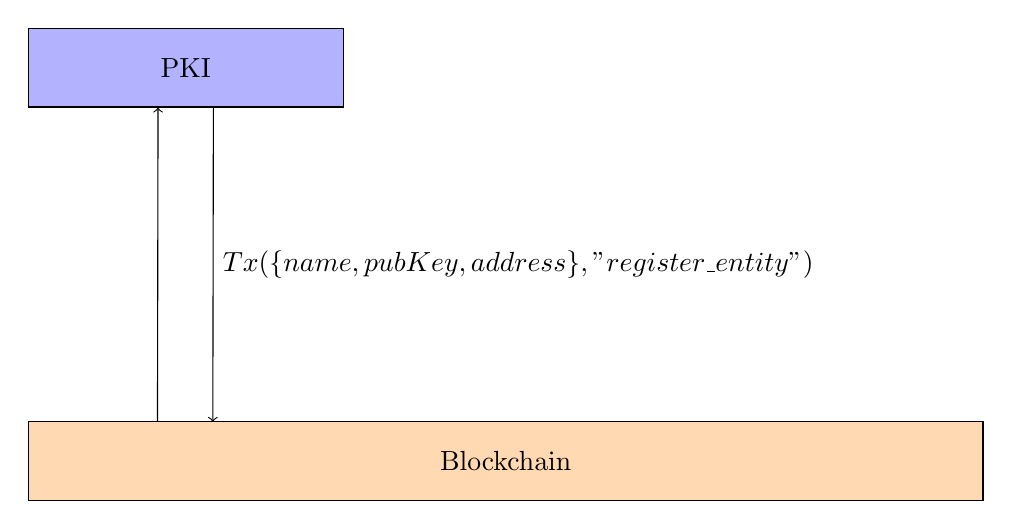
\begin{tikzpicture}
    \node[blockchain] (blockchain) at (0,0){Blockchain};

    \begin{scope}
      \node[node, anchor=west] (controller) at (0,5) {PKI};
      \draw[<-] ([xshift=-1em]controller.south) -- ([xshift=-1em]2,0.5);
      \draw[->] ([xshift=1em]controller.south) -- ([xshift=1em]2,0.5) node[midway,right] {$Tx(\{name, pubKey, address\}, "register\_entity")$};
    \end{scope}

  \end{tikzpicture}
  \caption{Entity Registration}
  \label{fig:arch:entity_reg}
\end{figure}

\section{Request for processing}
\label{solution:flow:pr_req}

A request for processing is the procedure where a participant of the network request a specific processing algorithm to be performed on a dataset of its choice. The requestor can only choose from datasets that are registered on the network and publicly available on the blockchain. A request for data processing is registered when the requestor sign and sent a request transaction to the blockchain. In its payload the public key of the requestor is included. The public key is needed by the processor to be able to encrypt data processing results as it crucial to be private from other parties. When a request is registered, a \verb|request| event is emitted notifying the interested parties. All data controllers are listening to \verb|request| events and are responsible for notifying a data processor for that request. The data controller, if the request concerns its dataset, selects randomly a data processor and encrypts the symmetric key of the dataset with its public key. The choice of the data processor could be also done sequentially; the data controller choose the next in line data processor. Selection by popularity in the existence of a decentralized ranking system is a another viable option. A transaction is sent to the blockchain to notify the selected data processor passing the id of the request and the encrypted symmetric key.

The request for processing procedure is summarized in Algorithm~\ref{alg:data_request}.

\begin{algorithm}[!htb]
  \caption{Request for processing}\label{alg:data_request}
  \begin{algorithmic}[1]
  \Function{\sf notify}{$e$}
    \State $p \rselect \{ p_1, p_2, \dots p_n \}$ \Comment{Select randomly processor}
    \Let{(requestID)}{e}
    \Let{tx}{(p)}
    \Let{(pk_p)}{tx.send()} \Comment{Get processor public key}
    \Let{c}{Enc_{pk_p}(k)} \Comment{Encrypt symmetric key}
    \Let{tx}{(requestID, c)} \Comment{Notify processor}
    \State $tx$.send()
    \State \Return{$tx$}
  \EndFunction
  \Procedure{\sf watch}{\null}
    \While{$e \in$ events['request']} \Comment{Listen data processing requests}
      \CommentLine{Check if the controller is the owner of the dataset}
      \If{isOwner($e$.datasetOwner)}
        \State notify($e$) \Comment{Notify processor}
      \EndIf
    \EndWhile
  \EndProcedure
  \Procedure{\sf request}{datasetID, algorithmID, $p_{k}$}
    \Let{tx}{(datasetID, algorithmID, p_{k})} \Comment{Request for processing}
    \State $tx$.send()
    \State \Return{$tx$}
  \EndProcedure
  \end{algorithmic}
\end{algorithm}

\begin{figure}[ht!]
  \begin{tikzpicture}

    \node[blockchain] (blockchain) at (0,0){Blockchain};

    \begin{scope}[node distance=4cm]
      \node[node, anchor=west] (owner) at (0,-5) {Data Controller};
      \draw[->] ([xshift=0em]owner.north) -- ([xshift=0em]2,-0.5);
    \end{scope}

    \node[txt] (list_req) [below=of owner, xshift=0em, yshift=1.5em] {$listen("request\_processing")$};

    \begin{scope}
      \node[node, anchor=west] (processor) at (0,5) {Data Processor};
      \draw[<-] ([xshift=0em]processor.south) -- ([xshift=0em]2,0.5) node[midway,right] {$Tx(\{requestID, Enc_{pk_P}(k)\}, "notify\_processor")$};
    \end{scope}

    \node[txt] (list_req_cr) [above=of processor, xshift=0em, yshift=-1.5em] {$listen("processing")$};

    \begin{scope}
      \node[node, anchor=east] (requester) at (\textwidth,-5) {Requester};
      \draw[->] ([xshift=0em]requester.north) -- ([xshift=0em]14.45,-0.5) node[midway,left] {\small $Tx(\{dataSetID, queryID, pubKey\}, "request\_processing")$};
    \end{scope}

  \end{tikzpicture}
  \caption{Request for processing}
  \label{fig:arch:req_pr}
\end{figure}

\section{Dataset processing}
\label{solution:flow:pr_data}

As it has already been mentioned in our study, the role of a data processor is crucial. By task assignments, it decrease the pressure over data controllers which they exploit them by entrusting specific data processing operations on behalf of data requestors. Data processors can only perform pre-agreed algorithms (§~\ref{solution:algorithms}) on datasets. Each processing must be accompanied by a proof of correctness of computation and an encrypted output which are published on the blockchain. A processor is constantly listening for \verb|process| events related to it. The controller notify the processor by emitting those events including the ID of the request and the encrypted symmetric key of the dataset. The processor, having all the needed information, signs a transaction to get the details of that request; the dataset ID and the algorithm ID. Another transaction is made to get the location and the hash of the dataset. As all informations are saved only in the blockchain, for traceability, accountability and provenance tracking to be enabled, those transactions are needed. The processor is ready to process the dataset. At first, it decrypts the symmetric key with its private key $sk_p$, downloads the dataset from the provided location and decrypts it. Assuming no errors, the computation is started and a proof, as analyzed in~\ref{solution:proof}, is generated with the evaluation key $ek_f$. The results are encrypted with the public key of the processor $pk_r$. Final, a transaction is sent to the blockchain with the proof $\pi$ and the encrypted results and an event is emitted to notify the requestor for the completion of the procedure.

The data processing procedure is summarized in Algorithm~\ref{alg:data_processing}.

\begin{algorithm}[!htb]
  \caption{Dataset processing}\label{alg:data_processing}
  \begin{algorithmic}[1]
  \Procedure{\sf process}{e}
    \Let{(\textsf{requestID}, \textsf{algorithmID}, c_{k}, pk_r)}{e}
    \Let{tx}{(\textsf{requestID})} \Comment{Get dataset id}
    \Let{(\textsf{datasetID}, \textsf{\textsf{algorithmID}})}{(tx)} \Comment{Get dataset info}
    \Let{(\textsf{location}, h)}{(tx)}
    \Let{k}{Dec_{sk_{p}}(c_{k})} \Comment{Decrypt symmetric key}
    \Let{c_{d}}{\textsf{get(location)}} \Comment{Get encrypted dataset}
    \Let{d}{Dec_{k}(c_{d})} \Comment{Decrypt dataset}
    \CommentLine{Process dataset and get proof of computation}
    \State $s \rselect{\{0, 1\}^{l}}$ \Comment{Salt generation with security parameter}
    \Let{F}{\textsf{algorithms['algorithmID']}}
    \Let{u}{(h, s)} \Comment{Public input}
    \Let{w}{d} \Comment{Private input}
    \Let{(\pi, \textsf{out})}{zkp(ek_f, F, u, w)} \Comment{Algorithm~\ref{alg:zkp}}
    \Let{tx}{(\pi, Enc_{pk_r}(\textsf{out}))} \Comment{Send results to requestor}
    \State $tx$.send()
  \EndProcedure
  \Procedure{\sf watch}{\null}
    \While{$e \in$ events['process']} \Comment{Listen data processing notifications}
      \State process($e$) \Comment{Process request}
    \EndWhile
  \EndProcedure
  \end{algorithmic}
\end{algorithm}

\section{Proof verification}
\label{solution:flow:verify}

The requestor, as zkSNARKs are non-interactive, can verify any time the correctness of the processing. It can either watch for \verb|process_done| events or by manually checking into the blockchain if a proof exists. Either way, is in its best interest to verify the proof. A transaction has again to be sent for request information retrieval. By sending the request ID the requestor gets the proof and the encrypted results. Then, it decrypts the results and verifies the proof with the verification key $vk_f$. In case of verification failure or the value of the \verb|valid| output variable is \verb|false| the proof is rejected.

The verification procedure is summarized in Algorithm~\ref{alg:data_verify}.

\begin{algorithm}[!htb]
  \caption{Proof verification}\label{alg:data_verify}
  \begin{algorithmic}[1]
  \Procedure{\sf verify}{e}
    \Let{(requestID)}{e}
    \Let{(\pi, c, \textsf{datasetID})}{tx(requestID).send()} \Comment{Get request info}
    \Let{h}{tx(datasetID).send()} \Comment{Get dataset info}
    \Let{(\pi, (y, h^{'}, s))}{Dec_{sk_{r}}(c)} \Comment{Decrypt results}
    \If{$h^{'}$ !== $h$} \Comment{Reject if digest not match}
      \State \textbf{reject}
    \EndIf
    \Let{valid}{\_verify(\pi, (y, h^{'}), (h, s), vk_f)} \Comment{Verify proof}
    \If{!valid} \Comment{Reject if not valid}
      \State \textbf{reject}
    \EndIf
  \EndProcedure
  \Procedure{\sf watch}{\null}
    \While{$e \in$ events['process\_done']} \Comment{Listen data processing completion}
      \State verify($e$) \Comment{Process request}
    \EndWhile
  \EndProcedure
  \end{algorithmic}
\end{algorithm}

\begin{figure}[ht!]
  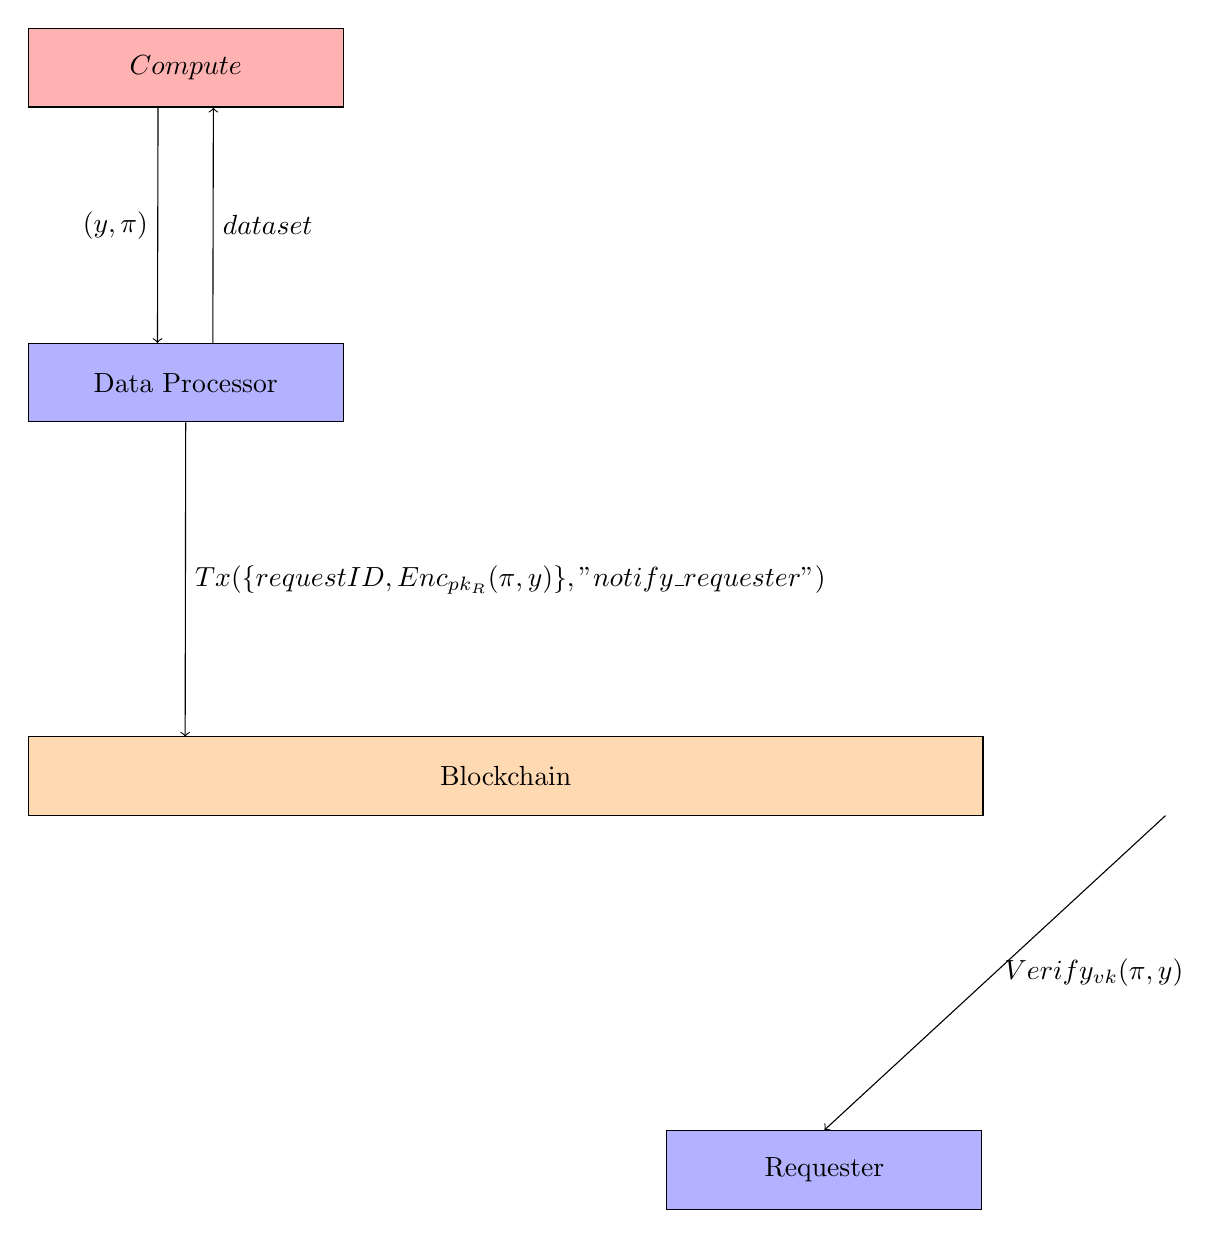
\begin{tikzpicture}

    \node[blockchain] (blockchain) at (0,0){Blockchain};

    \begin{scope}
      \node[node, anchor=west] (processor) at (0,5) {Data Processor};
      \draw[->] ([xshift=0em]processor.south) -- ([xshift=0em]2,0.5) node[midway,right] {$Tx(\{requestID, Enc_{pk_R}(\pi, y)\}, "notify\_requester")$};
    \end{scope}

    \node[node, process] (compute) [above of=processor, yshift=3cm] {$Compute$};

    \draw[->] ([xshift=-1em]compute.south) -- ([xshift=-1em]2,5.5) node[midway,left] {$(y, \pi)$};
    \draw[<-] ([xshift=1em]compute.south) -- ([xshift=1em]2,5.5)  node[midway,right] {$dataset$};

    \begin{scope}
      \node[node, anchor=east] (requester) at (\textwidth,-5) {Requester};
      \draw[<-] (requester.north) -- (14.45,-0.5) node[midway,right] {$Verify_{vk}(\pi, y)$};
    \end{scope}

  \end{tikzpicture}
  \caption{Data processing}
  \label{fig:arch:process}
\end{figure}

\begin{figure}[ht!]
  \begin{tikzpicture}

    \node[blockchain] (blockchain) at (0,0){Blockchain};

    \begin{scope}[node distance=4cm]
      \node[node, anchor=west] (owner) at (0,-5) {Data Controller};
      \node[database] (db) [below right=of owner] {Database};
      \draw[<->] (owner) -- (db) node[midway,left] {$Enc_k(data)$};
      \draw[<-] ([xshift=-1em]owner.north) -- ([xshift=-1em]2,-0.5);
      \draw[->] ([xshift=1em]owner.north) -- ([xshift=1em]2,-0.5) node[midway,right] {$Enc_{pk_P}(k, metadata)$};
    \end{scope}

    \begin{scope}
      \node[node, anchor=west] (processor) at (0,5) {Data Processor};
      \draw[<-] ([xshift=-1em]processor.south) -- ([xshift=-1em]2,0.5);
      \draw[->] ([xshift=1em]processor.south) -- ([xshift=1em]2,0.5) node[midway,right] {$Enc_{pk_R}(result, \pi)$};
    \end{scope}

    \begin{scope}
      \node[node, anchor=east] (requester) at (\textwidth,-5) {Requester};
      \draw[->] ([xshift=-1em]requester.north) -- ([xshift=-1em]14.45,-0.5) node[midway,left] {$Request(pk_R, pred)$};
      \draw[<-] ([xshift=1em]requester.north) -- ([xshift=1em]14.45,-0.5) node[midway,right]  {$Verify_{vk}(\pi)$};
    \end{scope}

  \end{tikzpicture}
  \caption{Architecture}
  \label{fig:architecture}
\end{figure}

%!TEX root = ../thesis.tex

\tikzstyle{database} = [cylinder, shape border rotate=90, aspect=0.5, draw, fill=green!30],
\tikzstyle{node} = [rectangle, minimum width=4cm, minimum height=1cm, text centered, draw=black, draw, fill=blue!30],
\tikzstyle{blockchain} = [draw,rectangle,minimum width=\textwidth, minimum height=1cm,anchor=west, fill=orange!30],
\tikzstyle{process} = [fill=red!30],
\tikzstyle{txt} = [],
\tikzstyle{entity} = [draw, minimum height=1cm, minimum width=4cm, fill=blue!30]
\tikzstyle{com} = [<->]
\tikzstyle{block} = [draw,thick,inner sep=10pt]
\tikzset{barstyle/.style 2 args={
      draw,
      minimum height=3em,
      fill=orange!30,
      fit={(#1.west) (#1.east)}, inner sep=0pt, label={center:#2}
    }
}

\chapter{Implementation}
\label{implemenation}

As mention at §~\ref{solution} the Blockchain act as the controller of the network. As a result, the application is separated in two parts. The off-chain network and the Blockchain network. The dataset storage, transmission and processing lives off-chain while dataset registration, requests for processing, processing outputs and Zero Knowledge proofs leave on the Blockchain. Every node on the network---a data share node--- is connected to the Blockchain and track every transaction specified for the application. That way it can track and index every registered dataset, request for processing and processing outputs and proofs and act accordingly.

\section{RESTful API}

A RESTful API is provided to facilitate communication between any application, that follows the REST architecture, and the data sharing Blockchain ecosystem. The REST API expose the blockchain business network that can be easily consumed by HTTP or REST clients. That way, any developer familiar with existing web technologies and frameworks is not obligated to learn the interval mechanisms of a Blockchain system to develop and deploy applications atop.

The REST API expose a set of routes each one having an HTTP method and a URI.

\begin{table}[ht!]
\centering
\begin{tabular}{|l|l|}
\hline
 Method & URI  \\ \hline
 GET & /\  \\ \hline
 GET &  /contracts \\ \hline
 GET &  /datastore \\ \hline
 GET &  /datastore/\{data\} \\ \hline
 POST &  /datastore\\ \hline
 GET &  /accounts \\ \hline
 GET &  /accounts/\{account\} \\ \hline
 GET &  /requests \\ \hline
 GET &  /requests/\{request\} \\ \hline
 POST &  /requests \\ \hline
 GET &  /processors \\ \hline
 POST &  /processors \\ \hline
\end{tabular}
\caption{RESTful API Routes}
\label{table:api_routes}
\end{table}

\section{Dapp}
\section{Processor}
\section{Controller}
\section{Command-line interface}
\section{Smart contracts}

\begin{figure}[ht!]
  \center
  \begin{tikzpicture}
    \begin{scope}[node distance=2cm]
      \node[entity] (api) {API};
      \node[entity] (dapp) [above=of api] {Dapp};
      \node[entity] (eth_node) [below=of api] {Ethereum node};
      \node[database] (db) [right=of api, yshift=-0.3cm] {Mongodb};
    \end{scope}

    \draw[com] (api) -- (eth_node);
    \draw[com] (api) -- (dapp);
    \draw[com] (api.east) ++ (right:0ex) -- ++ (right:2cm);

    \node[block,fit=(dapp) (eth_node) (db), label={Local Enviroment}] (local) {};

    \node[barstyle={local}{Ethereum Blockchain}, below=of local] (blockchain) {};

    \draw[com] (eth_node.south) ++ (south:0ex) -- ++ (south:1.35cm);

    \begin{scope}[node distance=2cm]
      \node[entity] (eth_node_pr) [below=of blockchain, xshift=-2cm, yshift=0.65cm] {Ethereum node};
      \node[entity] (processor) [below=of eth_node_pr] {Processor};
      \node[database] (db_pr) [right=of processor, yshift=-0.3cm] {Mongodb};
    \end{scope}

    \draw[com] (eth_node_pr.north) ++ (north:0ex) -- ++ (north:1.35cm);
    \draw[com] (processor) -- (eth_node_pr);
    \draw[com] (processor.east) ++ (right:0ex) -- ++ (right:2cm);

    \node[block,fit=(eth_node_pr) (processor) (db_pr), label={below:Local Enviroment}] (local) {};

  \end{tikzpicture}
  \caption{Implementation}
  \label{fig:implemenation}
\end{figure}

%!TEX root = ../thesis.tex
\chapter{Evaluation}
\label{evaluation}

We measure the efficiency of our solution via various analyses and comparisons. As storing data on Ethereum, and in blockchain in general, is expensive, the first series of experiments have been made regarding the cost of saving data by comparing and analyze various methods and alternatives. Second, we measure the cost of deploying the application on Ethereum and the cost of each of the individual operations. Lastly, a series of benchmarks have been made to measure the time and the size of computational proofs for each of the predefined algorithms supported by the data processors.

All experiments are conducted on MacBook Pro 2016 having a \verb|2GHz Intel Core i5| \verb|(2 cores)| CPU with \verb|8GB (1867 MHz LPDDR3)| of memory and a \verb|256GB PCI-Express SSD|. We use \verb|Ganache CLI v6.0.3 (ganache-core: 2.0.2)| as local Ethereum blockchain testnet and all smart contract are compiled with \verb|Solidity 0.4.19|.

\section{Benchmarks}
\label{evaluation:benchmarks}

\subsection{Data storage}
\label{evaluation:data_storage}

First, we measure the cost of storing raw data on the blockchain for each one of the following sizes: \verb|32 bytes|, \verb|1KB|, \verb|1MB|, \verb|10MB|, \verb|100MB| and \verb|1GB|. The size of \verb|32 bytes| is included as EVM words are of \verb|256-bits|. Table~\ref{table:bytes_usd_cost} reports the results.

As the size grows in multiples of ten the cost is growing significantly. Storing 1GB of data in Ethereum costs around 13.000.000 US dollars make it impossible and unpractical to store big data in blockchain. A common way of countermeasure is to store the data in an off-chain infrastructure (i.e IPFS~\cite{ipfs}, Storj~\cite{storj} or Filecoin~\cite{filecoin}) and store a reference to the data in the blockchain; a hash pointer. Storing a fixed size reference is much cheaper than saving an arbitrary size dataset. An alternative is to use the logging system of Ethereum whose cost of use is much cheaper than direct storage and can be used as an alternative for data storage.

In attempt to reduce storage costs, various experiments were conducted to compare different storage techniques. Four basic technique have been evaluated: data storage, data hash pointer storage, data logging, data hash pointer logging. Tables~\ref{table:data_store_comparison_01} to~\ref{table:data_store_comparison_05} shows the cost of the four possible ways of storing data for sizes of \verb|32 bytes|, \verb|1KB|, and \verb|1MB|. The size of hash value is constant and \verb|32 bytes|. Logging instead of saving the hash value to storage is cheaper by 35.42\%. Logging raw data far exceeds direct data storage by an average of 700\%.

At the time of the experiments the price of Ether is at 942.99 US dollars and the gas price is set at 2 Gwei.

\begin{table}[!htb]
\centering
\caption{Data storage costs.\\ ETH Price: \$942.99 (Feb 18, 2018) - Gas Price: 2 Gwei}
\begin{tabular}{|l|l|l|}
\hline
 Size & Gas  & USD \\ \hline
 32 bytes & 20.000  & \$0.037 \\ \hline
 1KB & 724.664  & \$1.357 \\ \hline
 1MB & 697.325.562  & \$1,305.393 \\ \hline
 10MB & 7.000.000.000  & \$13,104 \\ \hline
 100MB & 70.000.000.000  & \$131,040 \\ \hline
 1GB & 700.000.000.000  & \$13,104,000 \\ \hline
\end{tabular}
\captionsetup{format=hang, justification=centering}
\label{table:bytes_usd_cost}
\end{table}

\begin{figure}[!htb]
  \centering
  \begin{tikzpicture}
    \begin{axis}[xlabel=Gas,ylabel=Size]
      \addplot[
        color=red,
        mark=x
      ] coordinates {
        (0.032, 20000)
        (1, 724664)
        (1e+3, 697325562)
        (1e+4, 7e+10)
        (1e+5, 7e+11)
        (1e+6, 7e+12)
      };
    \end{axis}
  \end{tikzpicture}
  \captionsetup{format=hang, justification=centering}
  \caption{Data storage costs.\\ ETH Price: \$942.99 (Feb 18, 2018) - Gas Price: 2 Gwei}
  \label{fig:bytes_usd_cost}
\end{figure}

\begin{table}[!htb]
  \centering
  \captionsetup{format=hang, justification=centering}
  \caption{Comparing methods of data storage.\\ ETH Price: \$942.99 (Feb 18, 2018) - Gas Price: 2 Gwei - Data Size: 32 bytes}
  \begin{tabular}{|l|l|l|l|}
  \hline
  Type & Size & Gas  & USD \\ \hline
  Data storage & 32 bytes & 34.916  & \$0.065 \\ \hline
  Hash pointer storage & 32 bytes & 34.850  & \$0.065 \\ \hline
  Data logging & 32 bytes & 25.995  & \$0.048 \\ \hline
  Hash pointer logging & 32 bytes & 25.995  & \$0.048 \\ \hline
  \end{tabular}
  \label{table:data_store_comparison_01}
\end{table}

\begin{table}[!htb]
  \centering
  \captionsetup{format=hang, justification=centering}
  \caption{Comparing methods of data storage.\\ ETH Price: \$942.99 (Feb 18, 2018) - Gas Price: 2 Gwei - Data Size: 1KB}
  \begin{tabular}{|l|l|l|l|}
  \hline
    Type & Size & Gas  & USD \\ \hline
    Data storage & 1KB & 724.730  & \$1.347 \\ \hline
    Hash pointer storage & 32 bytes & 34.850  & \$0.065 \\ \hline
    Data logging & 1KB & 104.310  & \$0.194 \\ \hline
    Hash pointer logging & 32 bytes & 25.995  & \$0.048 \\ \hline
  \end{tabular}
  \label{table:data_store_comparison_02}
\end{table}

\begin{table}[!htb]
  \centering
  \captionsetup{format=hang, justification=centering}
  \caption{Comparing methods of data storage.\\ ETH Price: \$942.99 (Feb 18, 2018) - Gas Price: 2 Gwei - Data Size: 10KB}
  \begin{tabular}{|l|l|l|l|}
    \hline
      Type & Size & Gas  & USD \\ \hline
      Data storage & 10KB & 6.668.509  & \$12.39 \\ \hline
      Hash pointer storage & 32 bytes & 34.850  & \$0.065 \\ \hline
      Data logging & 10KB & 832.604  & \$1.547 \\ \hline
      Hash pointer logging & 32 bytes & 25.995  & \$0.048 \\ \hline
  \end{tabular}
  \label{table:data_store_comparison_03}
\end{table}

\begin{table}[!htb]
  \centering
  \captionsetup{format=hang, justification=centering}
  \caption{Comparing methods of data storage.\\ ETH Price: \$942.99 (Feb 18, 2018) - Gas Price: 2 Gwei - Data Size: 100KB}
  \begin{tabular}{|l|l|l|l|}
    \hline
    Type & Size & Gas  & USD \\ \hline
    Data storage & 100KB & 66.454.178  & \$123.472 \\ \hline
    Hash pointer storage & 32 bytes & 34.850  & \$0.065 \\ \hline
    Data logging & 100KB & 8.186.883  & \$15.211 \\ \hline
    Hash pointer logging & 32 bytes & 25.995  & \$0.048 \\ \hline
  \end{tabular}
  \label{table:data_store_comparison_04}
\end{table}

\begin{table}[!htb]
  \centering
  \captionsetup{format=hang, justification=centering}
  \caption{Comparing methods of data storage.\\ ETH Price: \$942.99 (Feb 18, 2018) - Gas Price: 2 Gwei - Data Size: 1MB}
  \begin{tabular}{|l|l|l|l|}
    \hline
    Type & Size & Gas  & USD \\ \hline
    Data storage & 1MB & 666.092.228  & \$1,237.599 \\ \hline
    Hash pointer storage & 32 bytes & 34.850  & \$0.065 \\ \hline
    Data logging & 1MB & 88.857.033  & \$165.096 \\ \hline
    Hash pointer logging & 32 bytes & 25.995  & \$0.048 \\ \hline
  \end{tabular}
  \label{table:data_store_comparison_05}
\end{table}

\begin{figure}[!ht]
\begin{subfigure}[t]{0.475\textwidth}
      \centering
      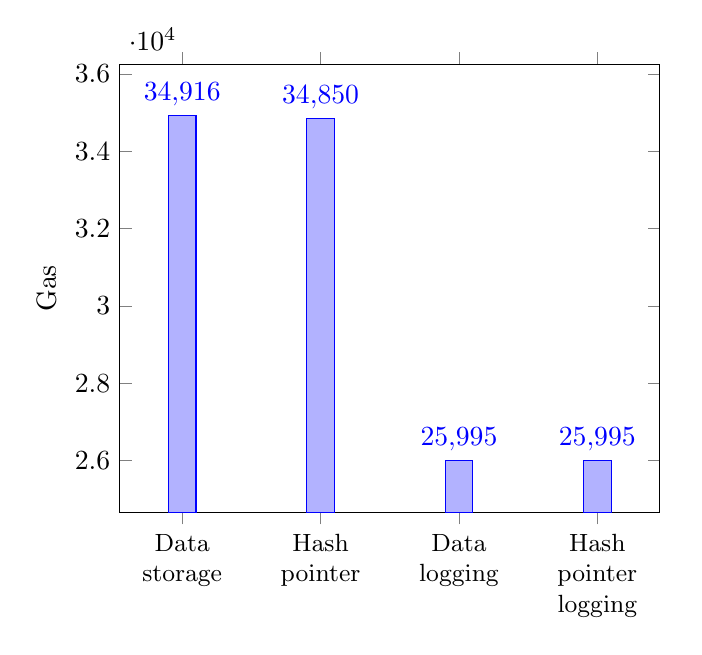
\begin{tikzpicture}
        \begin{axis}[bar]
          \addplot coordinates {
          (Data storage,34916)
          (Hash pointer,34850)
          (Data logging,25995)
          (Hash pointer logging, 25995)
          };
        \end{axis}
      \end{tikzpicture}
      \caption{Size: 32 bytes}
  \end{subfigure}
  \begin{subfigure}[t]{0.475\textwidth}
      \centering
      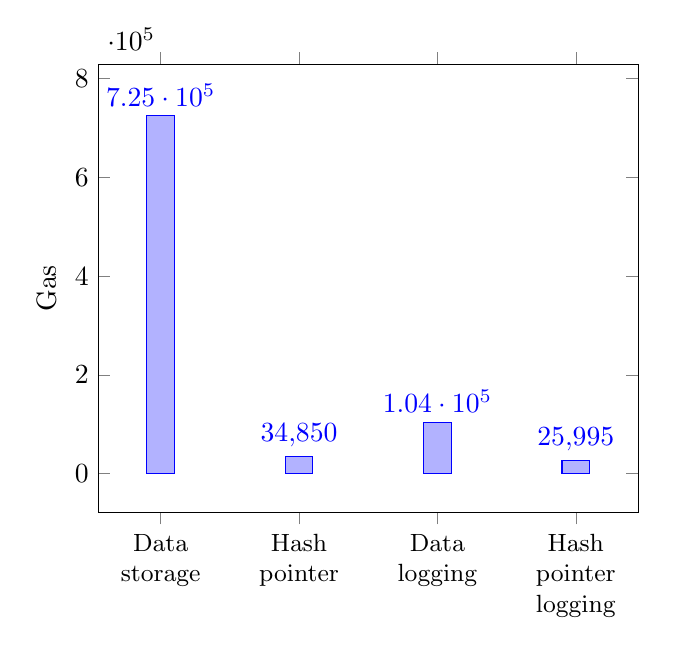
\begin{tikzpicture}
        \begin{axis}[bar]
          \addplot coordinates {
            (Data storage,724730)
            (Hash pointer,34850)
            (Data logging,104310)
            (Hash pointer logging, 25995)
          };
        \end{axis}
      \end{tikzpicture}
      \caption{Size: 1KB}
  \end{subfigure}
  \caption{Storage methods}
  \label{fig:storage:charts:01}
\end{figure}

\begin{figure}[!ht]
    \begin{subfigure}[t]{0.475\textwidth}
        \centering
        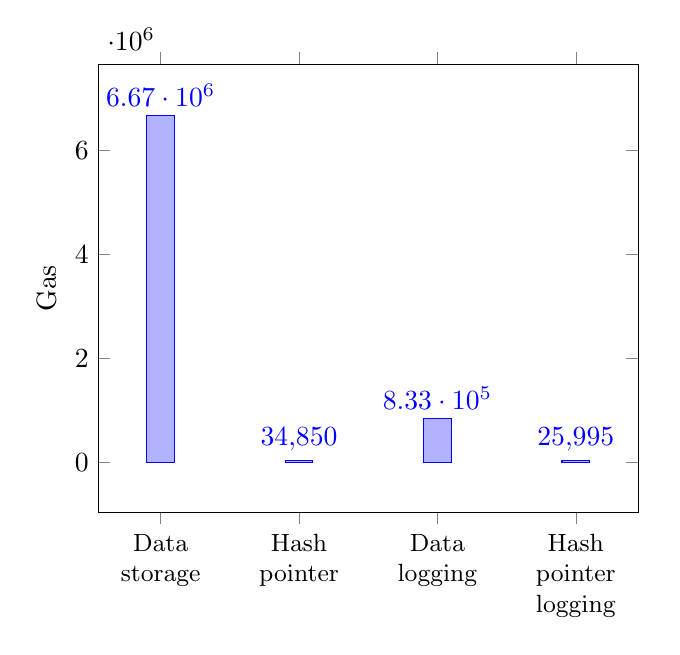
\begin{tikzpicture}
          \begin{axis}[bar]
            \addplot coordinates {
              (Data storage,6668509)
              (Hash pointer,34850)
              (Data logging,832604)
              (Hash pointer logging, 25995)
            };
          \end{axis}
        \end{tikzpicture}
        \caption{Size: 10KB}
    \end{subfigure}
    \begin{subfigure}[t]{0.475\textwidth}
        \centering
        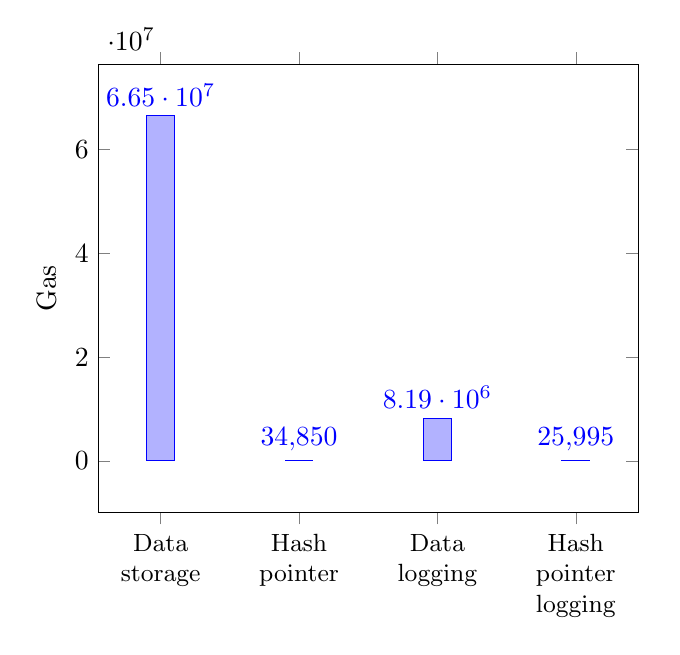
\begin{tikzpicture}
          \begin{axis}[bar]
            \addplot coordinates {
              (Data storage,66454178)
              (Hash pointer,34850)
              (Data logging,8186883)
              (Hash pointer logging, 25995)
            };
          \end{axis}
        \end{tikzpicture}
        \caption{Size: 100KB}
    \end{subfigure}
  \caption{Storage methods}
  \label{fig:storage:charts:02}
\end{figure}

\begin{figure}[!ht]
  \centering
  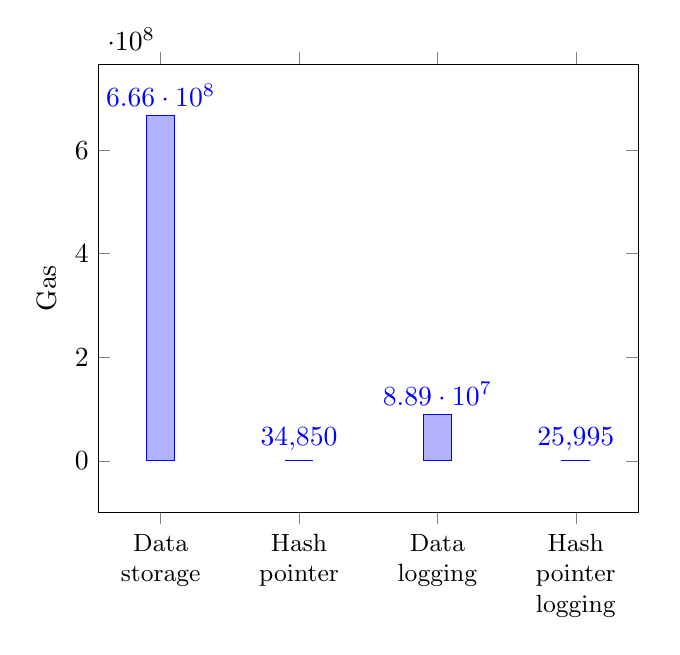
\begin{tikzpicture}
    \begin{axis}[bar]
      \addplot coordinates {
        (Data storage,666092228)
        (Hash pointer,34850)
        (Data logging,88857033)
        (Hash pointer logging, 25995)
      };
    \end{axis}
  \end{tikzpicture}
  \caption{Storage methods - Size: 1MB}
  \label{fig:storage:charts:1mb}
\end{figure}

\subsection{Application costs}
\label{evaluation:app_costs}

Each action by the participants has a cost in gas and therefore in money. Table~\ref{table:app_costs} shows the costs of each operation of the application. The most expensive operation is the dataset registration, with a cost of 233.487 gas, as it contains a lot of metadata for the dataset itself. Nevertheless, is an negligible cost considering the advantages of data sharing in privacy preserving manner.

\begin{table}[!htb]
\centering
\captionsetup{format=hang, justification=centering}
\caption{Application Costs.\\ ETH Price: \$942.99 (Feb 18, 2018) - Gas Price: 2 Gwei}
\begin{tabular}{|l|l|l|l|}
\hline
 Type & Gas & ETH & USD \\ \hline
 App deployment & 3.004.253 & 0.00601 & \$5.66 \\ \hline
 Register data set & 233.487 & 0.000467 & \$0.44 \\ \hline
 Request for processing & 89.206 & 0.0001784 & \$0.15 \\ \hline
 Register processor & 83.274 & 0.0001665 & \$0.15 \\ \hline
 Notify processor & 25.279 & 0.00005 & \$0.04 \\ \hline
\end{tabular}
\label{table:app_costs}
\end{table}

\subsection{Zero Knowledge Proofs}
\label{evaluation:zkp}

A series of benchmarks are performed to measure the performance of the basic parts of the construction and verification zero knowledge proofs. Proof generation is divided in three phases: \verb|Setup|, \verb|Compute| and \verb|Verify|. \verb|Setup| phase consists of the compilation of a \verb|C| programm to QAP (§~\ref{zkp:snarks}) and the generation of the keys needed for proof construction and verification. \verb|Setup| phase is executed once at application bootstrap and per processing algorithm. \verb|Compute| phase consists of circuit evaluation, polynomial solving and proof generation with the use of the evaluation key. Lastly, \verb|Verification| phase consists of proof verification by the verifier with the use of the verification key.

Tables~\ref{table:zkp_01} to~\ref{table:zkp_03} provide details of ZKP performance for each query that application supports and with inputs of size \verb|100|, \verb|1.000| and \verb|10.000|. For each query, we measure the time execution of each one of the three phases and the size of the generated keys and proofs. The keys are reasonably sized, with the evaluation key to typically be from 10 to 100 MB and the verification key to be 100KB. Due to the succinctness property of zkSNARKs the size of the proof is very small and constant for all programs regardless of input size. The size of the evaluation keys and the execution time of each one of the phases are proportional to program complexity.

\begin{table}[!htb]
\small
\centering
\captionsetup{format=hang, justification=centering}
\caption{ZKP Performance: 100 values}
\begin{tabular}{|l|l|l|l|l|l|l|}
\hline
 & Setup (s) & Compute (s) & Verify (ms) & Eval Key (MB) & Ver Key (KB) & Proof (B)  \\ \hline
 Sum & 10 & 8 & 28 & 0.016 & 100 & 304 \\ \hline
 Count & 16 & 8 & 26 & 0.005 & 100 & 304 \\ \hline
 Max & 17 & 9 & 28 & 1.7 & 100 & 304 \\ \hline
 Median & 65 & 30 & 28 & 64 & 100 & 304 \\ \hline
 Min & 17 & 9 & 51 & 1.7 & 100 & 304 \\ \hline
 Mean & 16 & 8 & 19 & 0.054 & 100 & 304 \\ \hline
\end{tabular}
\label{table:zkp_01}
\end{table}

\begin{table}[!htb]
\small
\centering
\captionsetup{format=hang, justification=centering}
\caption{ZKP Performance: 1.000 values}
\begin{tabular}{|l|l|l|l|l|l|l|}
\hline
 & Setup (s) & Compute (s) & Verify (ms) & Eval Key (MB) & Ver Key (KB) & Proof (B)  \\ \hline
 Sum & 10 & 8 & 27 & 0.144 & 100 & 304 \\ \hline
 Count & 15 & 9 & 37 & 0.036 & 100 & 304 \\ \hline
 Max & 29 & 14 & 34 & 17 & 100 & 304 \\ \hline
 Min & 28 & 14 & 49 & 17 & 100 & 304 \\ \hline
 Mean & 17 & 8 & 41 & 0.182 & 100 & 304 \\ \hline
 Median & 1701 & - & 12 & 64 & 100 & 304 \\ \hline
\end{tabular}
\label{table:zkp_02}
\end{table}

\begin{table}[!htb]
\small
\centering
\captionsetup{format=hang, justification=centering}
\caption{ZKP Performance: 10.000 values}
\begin{tabular}{|l|l|l|l|l|l|l|}
\hline
 & Setup (s) & Compute (s) & Verify (ms) & Eval Key (MB) & Ver Key (KB) & Proof (B)  \\ \hline
 Sum & 10 & 8 & 21 & 1.44 & 100 & 304 \\ \hline
 Count & 17 & 8 & 32 & 0.335 & 100 & 304 \\ \hline
 Max & 130 & 67 & 28 & 171 & 100 & 304 \\ \hline
 Min & 126 & 67 & 27 & 171 & 100 & 304 \\ \hline
 Mean & 22 & 9 & 27 & 1.5 & 100 & 304 \\ \hline
 Median & - & - & - & - & - & - \\ \hline
\end{tabular}
\label{table:zkp_03}
\end{table}

%!TEX root = ../thesis.tex
\chapter{Conclusion}
\label{conclusion}


\backmatter

\bibliography{./references} % Moved from class file due to cite autocomplete bugs with atom-latextools package

\end{document}
